%% chapter09_slides.tex
%% Four Variants of the Vehicle Routing Problem
%% Vehicle Routing: Problems, Methods, and Applications, 2nd ed. (2014)
%% Chapter 9 — Irnich, Schneider, Vigo
%% Self-contained lecture notes formatted as Beamer slides.
%%
%% Compile: pdflatex -interaction=nonstopmode chapter09_slides.tex (twice)

\documentclass[aspectratio=169,10pt]{beamer}

\usetheme{Madrid}
\usecolortheme{seahorse}

\usepackage{amsmath,amssymb,amsfonts}
\usepackage{booktabs}
\usepackage{graphicx}
\usepackage{listings}
\usepackage{xcolor}
\usepackage{tikz}
\usepackage{microtype}
\usepackage{array}
\usepackage{tabularx}
\usepackage{multirow}
\usepackage{hyperref}

\graphicspath{{figures/}}

\setbeamertemplate{footline}[frame number]
\setbeamertemplate{navigation symbols}{}

% listings style for Python
\lstset{
  language=Python,
  basicstyle=\ttfamily\scriptsize,
  numbers=left,
  numberstyle=\tiny\color{gray},
  frame=single,
  backgroundcolor=\color{gray!7},
  commentstyle=\color{green!50!black}\itshape,
  keywordstyle=\color{blue!80!black}\bfseries,
  stringstyle=\color{orange!70!black},
  breaklines=true,
  showstringspaces=false,
  tabsize=4,
}

%% ─── Title information ──────────────────────────────────────────────────────
\title[Ch.\,9: Four VRP Variants]{%
  Chapter 9: Four Variants of the\\
  Vehicle Routing Problem}
\subtitle{%
  \textit{Vehicle Routing: Problems, Methods, and Applications}\\
  2nd Edition (2014) — Irnich, Schneider \& Vigo}
\author{}
\date{}

%% ════════════════════════════════════════════════════════════════════════════
\begin{document}
%% ════════════════════════════════════════════════════════════════════════════

\begin{frame}
  \titlepage
\end{frame}

%%--------------------------------------------------------------------
\begin{frame}[allowframebreaks]{Chapter Overview}
  \begin{center}
    
\includegraphics[width=0.92\textwidth]{chapter_overview.pdf}
  \end{center}
\end{frame}

%%--------------------------------------------------------------------
\begin{frame}[allowframebreaks]{Table of Contents}
  \tableofcontents
\end{frame}

%% ════════════════════════════════════════════════════════════════════════════
\section{9.1 Introduction}
%% ════════════════════════════════════════════════════════════════════════════

\begin{frame}[allowframebreaks]{Introduction: Why Study VRP Variants?}

The classical Vehicle Routing Problem (VRP) asks us to find the cheapest set
of routes for a fleet of vehicles, all starting and ending at a central depot,
such that every customer is visited exactly once and no vehicle exceeds its
capacity.  In the real world, however, three additional features arise so
frequently that they have each generated their own substantial research
literature:

\begin{block}{Four Variants Covered in Chapter 9}
  \begin{enumerate}
    \item \textbf{VRP with Backhauls (VRPB)} --- customers are split into two
          groups: \emph{linehaul} customers who receive deliveries from the
          depot, and \emph{backhaul} customers from whom goods must be
          collected and brought back to the depot.  Because many vehicles can
          only be loaded from the rear, all deliveries must be completed before
          any pickups begin on the same route.
    \item \textbf{Heterogeneous or Mixed Fleet VRP (HFVRP)} --- the company
          operates vehicles of different sizes, each with its own capacity,
          fixed ownership cost, and per-kilometre variable cost.  Choosing
          \emph{which type} of vehicle to send is now part of the decision.
    \item \textbf{Periodic VRP (PVRP)} --- instead of a single day, planning
          spans several days ($T$ periods).  Each customer has a required
          \emph{visit frequency} (e.g.\ twice a week) and the planner must
          assign which specific days to visit and build efficient daily routes.
    \item \textbf{VRP with Split Deliveries (SDVRP)} --- the classical
          requirement that each customer is served by exactly one vehicle is
          relaxed.  A customer with a large demand may be served by two or more
          vehicles carrying partial loads, potentially reducing the total
          number of vehicles needed.
  \end{enumerate}
\end{block}

\framebreak

Each of these four families introduces a \emph{characteristic complication}
that makes the problem strictly harder than the basic VRP, yet each also
opens new algorithmic opportunities.  The variants are important both in
isolation and in combination: real logistics systems routinely combine, say,
periodic scheduling with a heterogeneous fleet.

\begin{alertblock}{Key Insight}
  None of these four variants is a trivial extension of the basic VRP.  Each
  requires specially tailored algorithms for effective solution.  The chapter
  surveys exact methods, classical heuristics, and modern metaheuristics for
  all four families, together with benchmark results that allow a reader to
  compare algorithmic performance.
\end{alertblock}

\end{frame}

%% ════════════════════════════════════════════════════════════════════════════
\section{9.2 VRP with Backhauls (VRPB)}
%% ════════════════════════════════════════════════════════════════════════════

\begin{frame}[allowframebreaks]{9.2 VRPB: Problem Definition}

In many distribution networks --- particularly grocery retail and
pharmaceutical distribution --- vehicles not only \emph{deliver} goods to
customers but also \emph{collect} empty bottles, recyclable packaging, or
returned merchandise on the same trip.  The two activities create an
important asymmetry: once the vehicle has started picking up goods, the
cargo area fills from the rear, making it impossible (or at least very
inconvenient) to deliver further goods stored deeper in the vehicle.

\begin{block}{Formal Definition}
  Let $V = \{0\} \cup L \cup B$ be the vertex set, where:
  \begin{itemize}
    \item vertex $0$ is the \textbf{depot},
    \item $L = \{1, \ldots, n_L\}$ is the set of \textbf{linehaul} customers
          (demand $d_i > 0$, meaning goods are \emph{delivered} to them),
    \item $B = \{n_L+1, \ldots, n_L+n_B\}$ is the set of \textbf{backhaul}
          customers (demand $d_i > 0$, meaning goods are \emph{collected} from
          them).
  \end{itemize}
  Each vehicle has capacity $Q$.  A feasible VRPB solution must satisfy:
  \begin{enumerate}
    \item Every linehaul customer in $L$ is visited exactly once.
    \item Every backhaul customer in $B$ is visited exactly once.
    \item On every route that serves both linehaul and backhaul customers,
          \textbf{all linehaul visits must come before any backhaul visit}
          (the precedence constraint).
    \item The total load on any vehicle (deliveries plus pickups considered
          separately) never exceeds $Q$.
  \end{enumerate}
\end{block}

\framebreak

\begin{block}{The Precedence Constraint --- Why It Exists}
  In practice, a vehicle's cargo area is often only accessible from the rear.
  When the vehicle leaves the depot it is fully loaded with goods for linehaul
  customers; these are stacked from the front.  If the driver tried to pick up
  backhaul goods first, they would need to rearrange the entire load --- an
  operation that is either physically impossible or so time-consuming as to be
  uneconomic.  The precedence constraint models this physical reality:

  \[
    \text{if route } r \text{ visits both linehaul and backhaul customers,}
    \quad \text{then } i \in L \text{ appears before } j \in B \text{ in route } r.
  \]
\end{block}

\begin{alertblock}{Key Insight}
  The VRPB belongs to the broader class of \emph{Delivery and Collection VRP}.
  Combining both activities in one route is more efficient than running
  separate delivery and collection tours, but the precedence constraint
  restricts how much the routes can be interleaved.
\end{alertblock}

\end{frame}

%%--------------------------------------------------------------------
\begin{frame}[allowframebreaks]{VRPB: Three Structural Variants}

The literature distinguishes three ways in which linehaul ($L$) and backhaul
($B$) customers can coexist on a route.  Relaxing the strict precedence
constraint leads to progressively easier (but still NP-hard) problems.

\begin{center}
  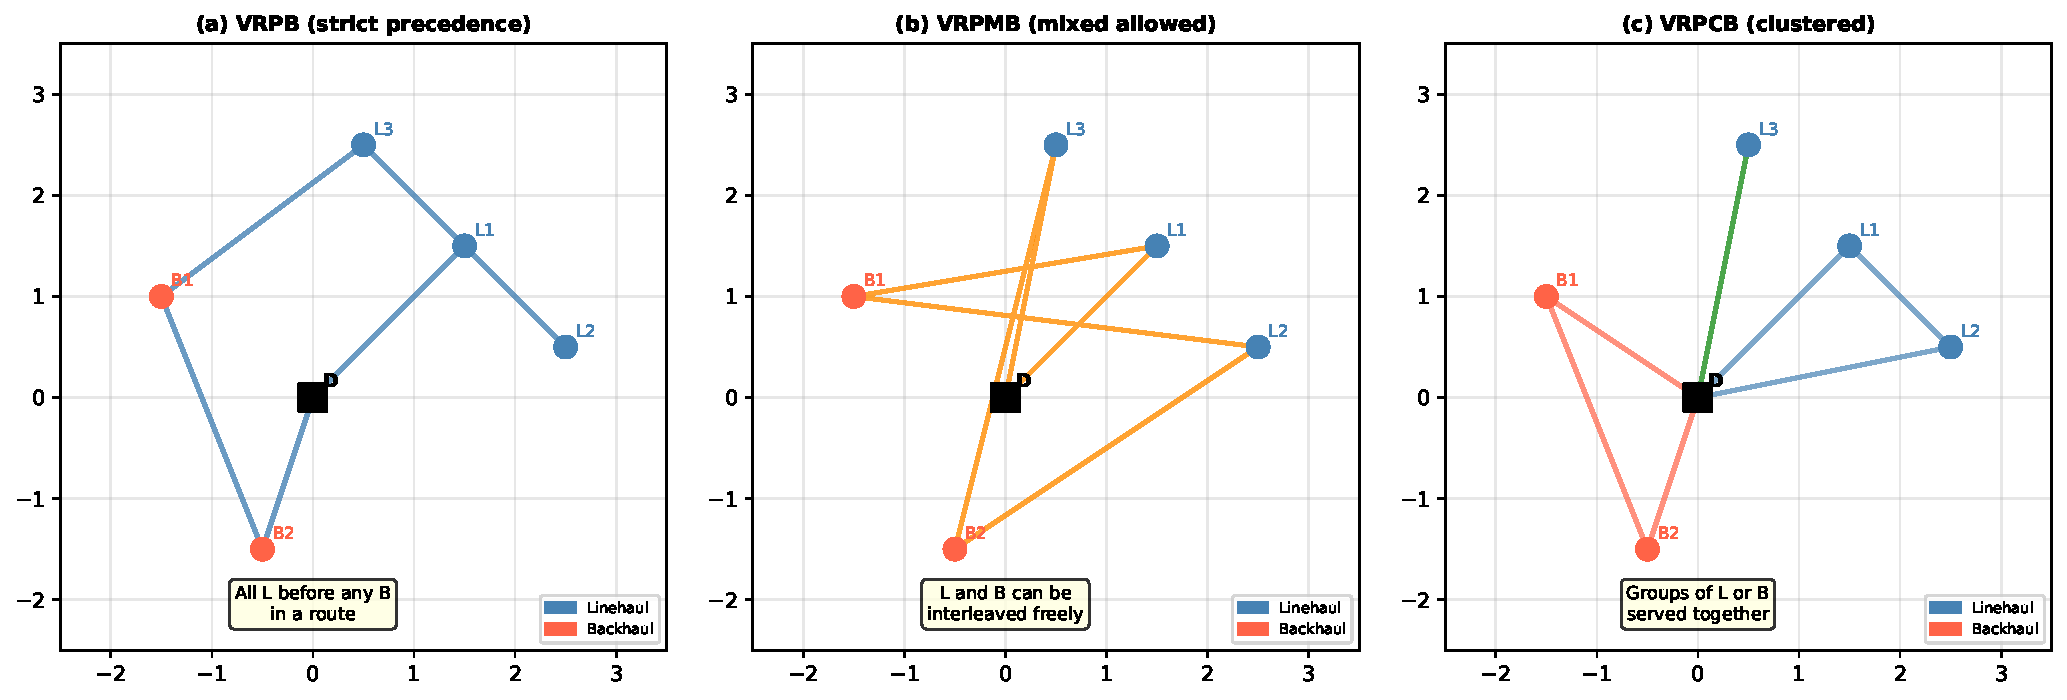
\includegraphics[width=0.90\textwidth]{vrpb_variants.pdf}
\end{center}

\begin{block}{(a) Classical VRPB --- Strict Precedence}
  All linehaul customers on a route are served before any backhaul customer.
  This corresponds to the physical loading constraint described above.  Mixing
  linehaul and backhaul sequences is simply \emph{forbidden}.
\end{block}

\begin{block}{(b) Mixed VRPB (VRPMB) --- Interleaving Allowed}
  The precedence constraint is dropped: a route may alternate freely between
  linehaul and backhaul customers.  This is feasible if the vehicle can be
  loaded from both ends, or if a forklift is available at each stop.  The
  VRPMB is generally easier to solve because it admits a larger feasible set.
\end{block}

\begin{block}{(c) Clustered VRPB (VRPCB) --- Grouped Visits}
  Linehaul and backhaul customers are served in \emph{clusters}: a sub-route
  visits a group of linehaul customers, then the vehicle may return to the
  depot (or proceed to a backhaul cluster).  This is a compromise between
  strict and mixed variants.
\end{block}

\end{frame}

%%--------------------------------------------------------------------
\begin{frame}[allowframebreaks]{VRPB: Route Feasibility and Load Tracking}

Understanding how the vehicle load changes along a VRPB route is essential
for checking feasibility.  Consider a route serving linehaul customers
$\ell_1, \ell_2, \ldots, \ell_p$ followed by backhaul customers
$b_1, b_2, \ldots, b_q$.

\begin{block}{Load Evolution on a Feasible VRPB Route}
  Let $Q$ denote the vehicle capacity, $d_i$ the demand of customer $i$.
  The vehicle starts at the depot with load $\sum_{j=1}^{p} d_{\ell_j}$
  (carrying all linehaul deliveries).  The load \emph{decreases} as linehaul
  deliveries are made, then \emph{increases} as backhaul pickups are made:
  \[
    \text{Load after serving } \ell_k = \sum_{j=1}^{p} d_{\ell_j}
                                        - \sum_{j=1}^{k} d_{\ell_j}
                                      = \sum_{j=k+1}^{p} d_{\ell_j}.
  \]
  After the last linehaul customer, the load reaches its minimum.  Then:
  \[
    \text{Load after serving } b_k = \sum_{j=1}^{k} d_{b_j}.
  \]
  Feasibility requires:
  \[
    \sum_{j=1}^{p} d_{\ell_j} \leq Q \quad \text{(capacity at departure)}
    \qquad \text{and} \qquad
    \sum_{j=1}^{q} d_{b_j} \leq Q \quad \text{(capacity on return)}.
  \]
\end{block}

\begin{exampleblock}{Worked Example: Load Tracking}
  Suppose $Q = 15$.  Linehaul customers have demands $d_{L1}=4,\, d_{L2}=5,\,
  d_{L3}=3$ (total = 12).  Backhaul customers have demands $d_{B1}=6,\,
  d_{B2}=7$ (total = 13).
  \begin{itemize}
    \item \textbf{At depot}: load = 12 (carrying $4+5+3$). Feasible: $12 \leq 15$.
    \item \textbf{After L1}: load = $12 - 4 = 8$.
    \item \textbf{After L2}: load = $8 - 5 = 3$.
    \item \textbf{After L3}: load = $3 - 3 = 0$ (vehicle now empty).
    \item \textbf{After B1}: load = $0 + 6 = 6$.
    \item \textbf{After B2}: load = $6 + 7 = 13 \leq 15$. Feasible.
  \end{itemize}
  Both the delivery and pickup loads satisfy the capacity constraint, so this
  route is feasible.
\end{exampleblock}

\end{frame}

%%--------------------------------------------------------------------
\begin{frame}[allowframebreaks]{VRPB: Mathematical Formulation}

The VRPB can be modelled as an integer program.  We define a complete directed
graph $G = (V, A)$ where $V = \{0\} \cup L \cup B$ and $A$ is the set of
all arcs.

\begin{block}{Decision Variables and Parameters}
  \begin{itemize}
    \item $c_{ij}$ --- travel cost (distance or time) from node $i$ to node $j$.
    \item $x_{ij} \in \{0,1\}$ --- equals 1 if some vehicle travels arc
          $(i,j)$, and 0 otherwise.  (Here $x_{ij}$ is read ``x sub i j.'')
    \item $m$ --- number of available vehicles.
    \item $d_i$ --- demand of customer $i$ (delivery amount for $i \in L$,
          pickup amount for $i \in B$).
    \item $Q$ --- vehicle capacity (maximum load it can carry).
    \item $u_i$ --- auxiliary variable used to eliminate sub-tours.
  \end{itemize}
\end{block}

\begin{block}{Objective Function}
  \[
    \min \sum_{(i,j) \in A} c_{ij} x_{ij}
  \]
  This formula says: minimise the total travel cost summed over all arcs
  actually used (i.e.\ all arcs where $x_{ij}=1$).  Increasing $c_{ij}$
  for a long arc makes the model prefer shorter routes.
\end{block}

\framebreak

\begin{block}{Constraints}
  \textbf{Degree constraints} (every customer visited exactly once):
  \[
    \sum_{j \in V} x_{ij} = 1 \quad \forall\, i \in L \cup B
    \qquad \text{(each customer has exactly one outgoing arc)}
  \]
  \[
    \sum_{i \in V} x_{ij} = 1 \quad \forall\, j \in L \cup B
    \qquad \text{(each customer has exactly one incoming arc)}
  \]

  \textbf{Fleet size} (depot degree):
  \[
    \sum_{j \in L} x_{0j} \leq m
    \qquad \text{(at most $m$ routes depart from the depot)}
  \]

  \textbf{Precedence constraint} (linehaul before backhaul):
  For every arc $(i,j)$ with $i \in B$ and $j \in L$, we set $x_{ij}=0$.
  Equivalently, no arc may go from a backhaul node directly to a linehaul node.

  \textbf{Capacity constraints}:
  Using sub-tour elimination variables $u_i$ (MTZ formulation):
  \[
    u_i - u_j + Q \cdot x_{ij} \leq Q - d_j \quad \forall\, i,j \in V,\, i \neq j
  \]
  \[
    d_i \leq u_i \leq Q \quad \forall\, i \in V \setminus \{0\}
  \]
  Here $u_i$ tracks the cumulative load \emph{up to} node $i$ and prevents
  both sub-tours and capacity violations.
\end{block}

\begin{alertblock}{How to Read This Formulation}
  The objective minimises total distance driven.  The degree constraints
  ensure every customer is visited exactly once.  The precedence constraint
  directly forbids the ``wrong order'' arcs.  The MTZ constraints elegantly
  combine sub-tour elimination with capacity tracking in a single set of
  inequalities.
\end{alertblock}

\end{frame}

%%--------------------------------------------------------------------
\begin{frame}[allowframebreaks]{VRPB: Exact Methods}

Exact methods for VRPB guarantee finding the globally optimal solution but
are computationally expensive.  The two main approaches are
\textbf{Branch-and-Bound} and \textbf{Column Generation} (Branch-and-Price).

\begin{block}{Branch-and-Bound for VRPB}
  The Branch-and-Bound (B\&B) approach works as follows.  Start by solving the
  \emph{Linear Programming relaxation} (LP) of the ILP --- this gives a lower
  bound on the optimal integer solution.  If the LP solution contains
  fractional $x_{ij}$ values, we \emph{branch}: fix one fractional variable
  to 0 or 1 and solve two sub-problems.  This creates a binary search tree;
  at each node we compute bounds and prune branches that cannot improve the
  current best integer solution.

  \medskip
  For VRPB, the first exact approach was proposed by \textbf{Goetschalckx
  and Jacobs-Blecha (1989)}, who used a set-partitioning formulation.  The
  method can solve instances with up to 70 customers to optimality.
\end{block}

\begin{block}{Branch-and-Price (Column Generation)}
  A more powerful exact approach decomposes the problem into:
  \begin{itemize}
    \item \textbf{Master problem}: select a subset of pre-generated routes
          (columns) with minimum total cost such that every customer is
          covered.
    \item \textbf{Pricing sub-problem}: find new routes (columns) with
          negative reduced cost that should be added to the master problem.
          For VRPB, this is a \emph{constrained shortest path problem} that
          respects the precedence constraint.
  \end{itemize}
  Toth and Vigo extended B\&P to handle both VRP and VRPB.  Using
  \textbf{Valid Inequalities} (capacity cuts, precedence cuts) dramatically
  tightens the LP bound.
\end{block}

\framebreak

\begin{block}{Computational Complexity}
  The VRPB is NP-hard (it contains VRP as a special case when $B = \emptyset$).
  In practice:
  \begin{itemize}
    \item Exact B\&B can handle $|L|+|B| \lesssim 50$ customers.
    \item Branch-and-Price pushes this to $|L|+|B| \lesssim 100$ customers.
    \item Beyond this, heuristic methods are essential.
  \end{itemize}
\end{block}

\begin{block}{Benchmark: Toth and Vigo (1997) Results}
  On the standard VRPB benchmark set (Goetschalckx--Jacobs-Blecha instances,
  $n \leq 100$ customers):
  \begin{itemize}
    \item B\&P solves most instances to optimality within minutes.
    \item Instances with $n = 100$ may require several hours.
    \item The LP lower bound is typically within 3--5\% of the optimum.
  \end{itemize}
\end{block}

\end{frame}

%%--------------------------------------------------------------------
\begin{frame}[allowframebreaks]{VRPB: Heuristics}

Because exact methods are too slow for large instances, a rich collection of
heuristics has been developed for VRPB.  The most important ones are
adaptations of classical VRP heuristics that respect the precedence
constraint.

\begin{block}{Clarke-Wright Savings Heuristic (Adapted for VRPB)}
  The \textbf{savings algorithm} (Clarke and Wright, 1964) starts with a
  ``star'' solution in which each customer has its own dedicated route:
  Depot $\to$ customer $i$ $\to$ Depot.  It then merges pairs of routes
  by computing the \emph{saving} $s(i,j) = c_{0i} + c_{j0} - c_{ij}$:
  the distance saved by linking customer $i$ to customer $j$ instead of
  returning to the depot between them.

  \medskip
  The saving says: instead of travelling Depot$\to i \to$ Depot$\to j \to$
  Depot (cost $c_{0i}+c_{i0}+c_{0j}+c_{j0}$), travel Depot$\to i \to j \to$
  Depot (cost $c_{0i}+c_{ij}+c_{j0}$).  The saving is $c_{i0}+c_{0j}-c_{ij}$.

  \medskip
  For VRPB, the savings algorithm must additionally ensure:
  \begin{enumerate}
    \item Merging two routes never creates a backhaul-before-linehaul sequence.
    \item The combined load does not exceed $Q$.
  \end{enumerate}
  In practice, this means linehaul customers are merged first, then backhaul
  customers, and only feasible merges are accepted.
\end{block}

\framebreak

\begin{exampleblock}{Worked Example: VRPB Savings Algorithm}
  Consider depot $D=(0,0)$ and 4 customers with Euclidean distances:
  \begin{center}
  \begin{tabular}{lrrrrrr}
    \toprule
    & $D$ & $L1$ & $L2$ & $B1$ & $B2$ \\
    \midrule
    $D$  & 0 & 3.6 & 2.8 & 2.2 & 3.2 \\
    $L1$ & 3.6 & 0 & 2.0 & 4.5 & 5.0 \\
    $L2$ & 2.8 & 2.0 & 0 & 3.1 & 4.2 \\
    $B1$ & 2.2 & 4.5 & 3.1 & 0 & 1.4 \\
    $B2$ & 3.2 & 5.0 & 4.2 & 1.4 & 0 \\
    \bottomrule
  \end{tabular}
  \end{center}

  Vehicle capacity $Q=10$; demands: $L1=4, L2=5, B1=3, B2=4$.

  \medskip
  \textbf{Step 1.}  Initial solution: 4 separate routes, total cost
  $= 2(3.6+2.8+2.2+3.2) = 23.6$.

  \medskip
  \textbf{Step 2.}  Compute savings for linehaul pairs:
  \[s(L1,L2) = 3.6+2.8-2.0 = 4.4 \quad \text{(best!)}
  \]
  Merge $L1$ and $L2$: route $D \to L1 \to L2 \to D$, load $=9 \leq 10$.

  \medskip
  \textbf{Step 3.}  Compute savings for backhaul pairs:
  \[s(B1,B2) = 2.2+3.2-1.4 = 4.0 \quad \text{(best!)}
  \]
  Merge $B1$ and $B2$: route $D \to B1 \to B2 \to D$, load $=7 \leq 10$.

  \medskip
  \textbf{Step 4.}  Try combining routes: can we add backhauls to the linehaul
  route?  Combined load $= 9+7=16 > Q=10$.  Not feasible.

  \medskip
  \textbf{Final solution}: Route 1: $D \to L1 \to L2 \to D$ (cost $=3.6+2.0+2.8=8.4$);
  Route 2: $D \to B1 \to B2 \to D$ (cost $=2.2+1.4+3.2=6.8$).
  Total cost $= 15.2$ (saving of $8.4$ vs.\ initial).
\end{exampleblock}

\end{frame}

%%--------------------------------------------------------------------
\begin{frame}[allowframebreaks]{VRPB: Metaheuristics}

For large instances (hundreds of customers), metaheuristics that intelligently
explore the solution space are the method of choice.

\begin{block}{Tabu Search for VRPB}
  \textbf{Tabu Search (TS)} is a local search method that accepts moves even
  when they temporarily worsen the solution, to escape local optima.  It
  maintains a \emph{tabu list} of recently visited solutions (or recently made
  moves) and forbids revisiting them for a fixed number of iterations.

  \medskip
  For VRPB, Tabu Search operators include:
  \begin{itemize}
    \item \textbf{Customer relocation}: move a single customer from one route
          to another (checking precedence and capacity).
    \item \textbf{2-opt}: reverse a segment of a route.  Only applicable if
          the resulting route still has all linehaul before all backhaul.
    \item \textbf{Or-opt}: move a chain of 1, 2, or 3 consecutive customers
          to another position in any route.
    \item \textbf{Cross-exchange}: swap segments between two routes.
  \end{itemize}
  The most effective published TS for VRPB is due to \textbf{Toth and Vigo
  (1997)}, achieving solutions within 1--2\% of the best known on benchmark
  instances.
\end{block}

\framebreak

\begin{block}{Genetic Algorithms (GA) for VRPB}
  A Genetic Algorithm maintains a \emph{population} of solutions (``chromosomes'').
  At each generation it selects parent solutions by fitness (total cost),
  applies \emph{crossover} to combine parents into offspring, and applies
  \emph{mutation} to introduce new material.  For VRPB:
  \begin{itemize}
    \item \textbf{Chromosome encoding}: a permutation of customers with
          position-based encoding; backhaul customers are always placed after
          linehaul customers in each route segment.
    \item \textbf{Crossover}: Order Crossover (OX) preserves the relative
          order of customers from one parent while copying a segment from the
          other parent.
    \item \textbf{Repair operator}: after crossover, a feasibility check
          ensures the precedence constraint holds; violations are fixed by
          moving misplaced customers.
  \end{itemize}
  Validating benchmark results, GAs reach solutions of comparable quality to
  TS in similar or shorter times, but are more sensitive to parameter tuning.
\end{block}

\begin{block}{Adaptive Large Neighbourhood Search (ALNS)}
  ALNS (Ropke and Pisinger, 2006) is among the most competitive methods for
  VRP variants.  It repeatedly \emph{destroys} part of the current solution
  (removing a random subset of customers) and \emph{repairs} it (re-inserting
  removed customers optimally).  Destroy and repair operators are selected
  adaptively: operators that have historically produced good solutions are
  chosen more frequently.  For VRPB, the repair step must respect the
  precedence constraint when re-inserting backhaul customers.
\end{block}

\end{frame}

%%--------------------------------------------------------------------
\begin{frame}[allowframebreaks]{VRPB: Route Diagram and Summary}

\begin{center}
  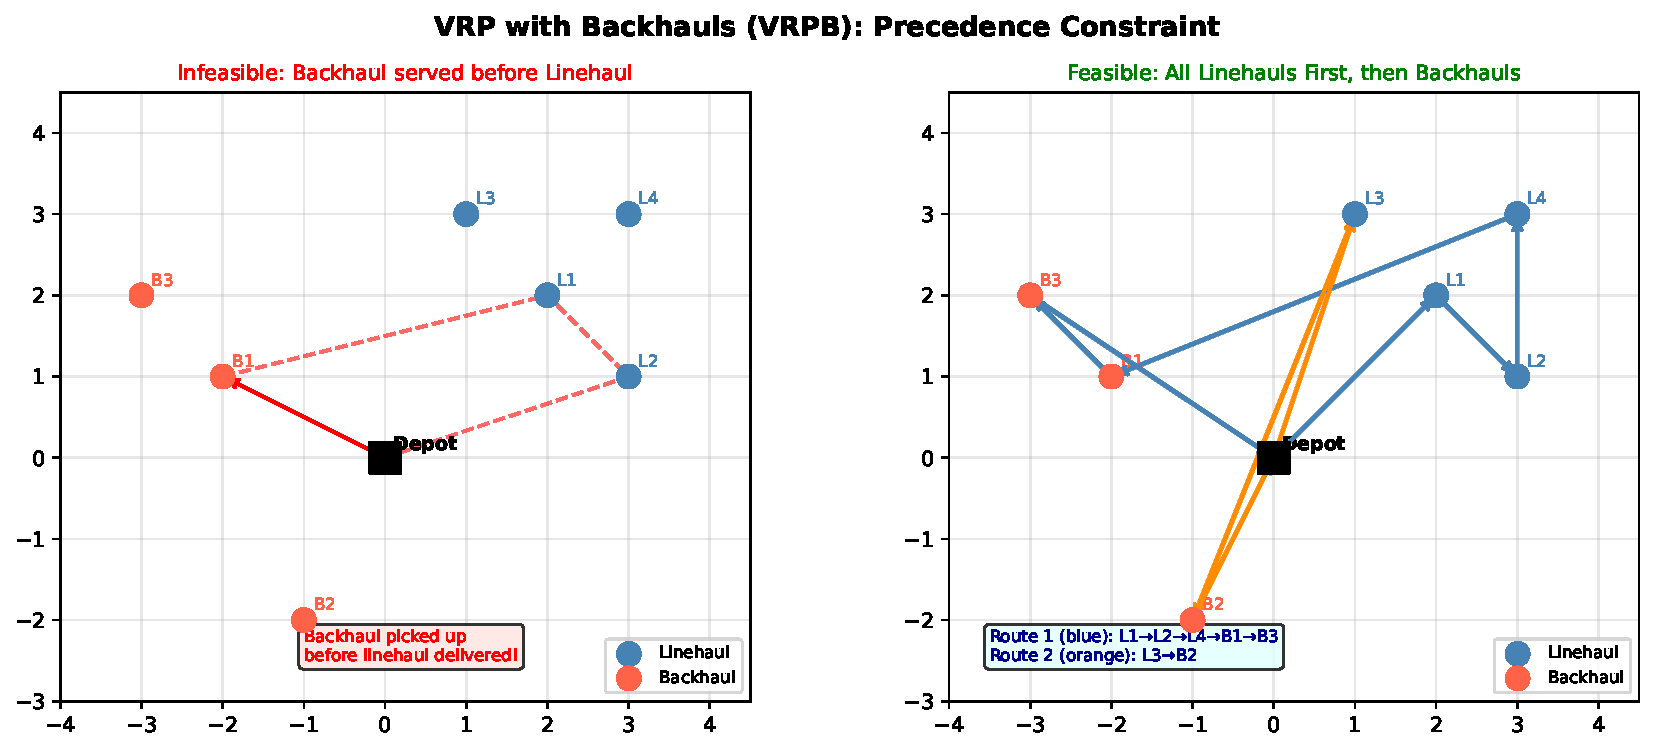
\includegraphics[width=0.90\textwidth]{vrpb_routes.pdf}
\end{center}

The left panel shows an \emph{infeasible} route where a backhaul customer is
served before linehaul customers --- this violates the precedence constraint.
The right panel shows two feasible routes: Route 1 (blue) serves linehaul
customers $L1, L2, L4$ before backhaul customers $B1, B3$; Route 2 (orange)
serves $L3$ before $B2$.

\begin{alertblock}{VRPB Summary}
  The VRP with Backhauls models the practical reality that vehicles often both
  deliver and collect on the same trip.  The precedence constraint (linehaul
  before backhaul) reflects vehicle loading geometry.  Exact methods using
  B\&P solve instances up to $\approx100$ customers.  For larger instances,
  metaheuristics such as Tabu Search and ALNS achieve solutions within 1--3\%
  of the best known.
\end{alertblock}

\end{frame}

%% ════════════════════════════════════════════════════════════════════════════
\section{9.3 Heterogeneous or Mixed Fleet VRP (HFVRP)}
%% ════════════════════════════════════════════════════════════════════════════

\begin{frame}[allowframebreaks]{9.3 HFVRP: Problem Definition and Variants}

In the classical VRP, all vehicles are assumed identical: same capacity, same
fuel consumption, same fixed cost.  In practice, almost every real fleet is
\emph{heterogeneous}: a logistics company might operate motorcycles for small
express deliveries alongside 40-tonne articulated lorries for bulk shipments.
The Heterogeneous Fleet VRP (HFVRP) --- also called Mixed Fleet VRP or Free
Fleet Size and Mix VRP --- explicitly models this diversity.

\begin{block}{Problem Setting}
  There are $T$ vehicle \emph{types}, indexed $t = 1, \ldots, T$.  Each type
  $t$ is characterised by:
  \begin{itemize}
    \item $Q_t$ --- capacity (maximum load it can carry per trip),
    \item $f_t$ --- fixed cost per vehicle used (ownership or daily rental cost),
    \item $r_t$ --- variable cost per unit of distance travelled.
  \end{itemize}
  There may be $m_t$ vehicles of type $t$ available (fixed fleet size case),
  or the fleet size may be unlimited (free fleet size case, FSMVRP).  The
  goal is to assign vehicle types to routes and find routes that minimise
  total cost (fixed + variable).
\end{block}

\framebreak

\begin{block}{HFVRP Sub-Families (Table 9.1 in the Book)}
  \begin{center}
    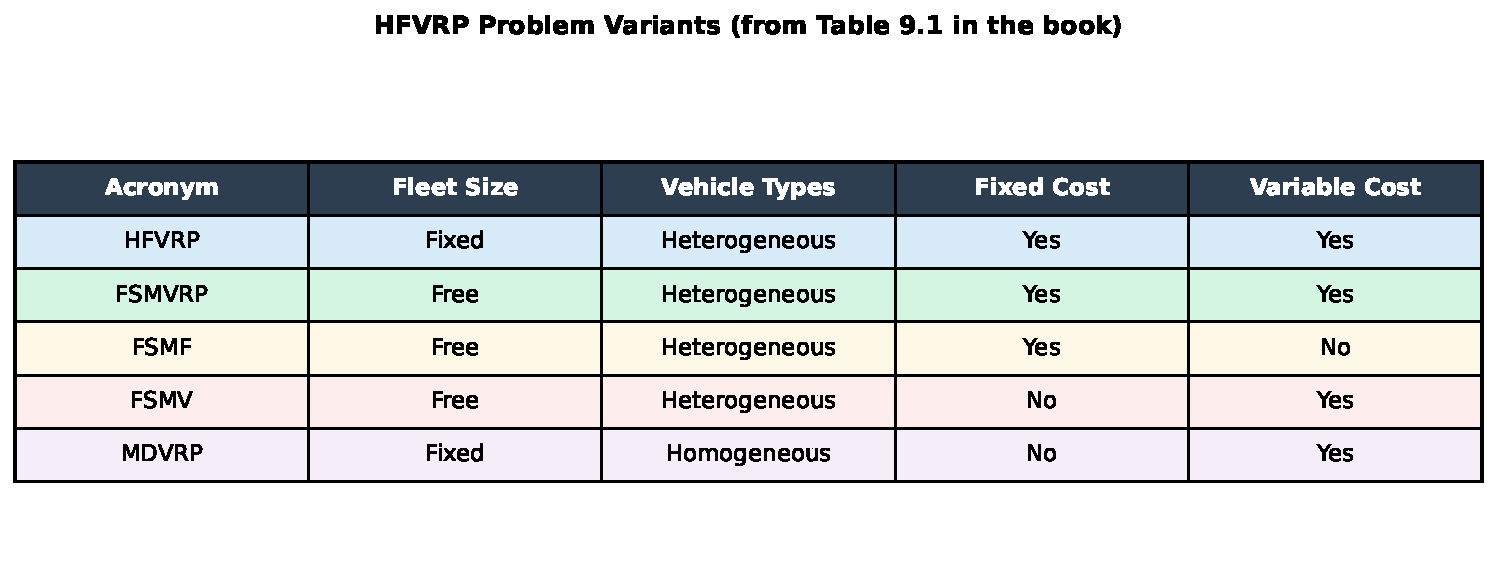
\includegraphics[width=0.80\textwidth]{hfvrp_variants_table.pdf}
  \end{center}
  The key distinction is between \textbf{fixed fleet} (HFVRP: you must use
  exactly the vehicles you have) and \textbf{free fleet} (FSMVRP: you choose
  how many of each type to use).  In the free-fleet case, using many small
  vehicles trades lower capacity per vehicle for lower fixed costs (if small
  vehicles are cheaper to own).
\end{block}

\begin{alertblock}{Key Insight: The Vehicle-Assignment Decision}
  Adding vehicle-type selection makes HFVRP strictly harder than VRP: we must
  simultaneously decide \emph{which type} of vehicle to send and \emph{which
  route} it should take.  This creates a more complex optimisation landscape.
\end{alertblock}

\end{frame}

%%--------------------------------------------------------------------
\begin{frame}[allowframebreaks]{HFVRP: Mathematical Formulation}

Let $G = (V, A)$ with $V = \{0,1,\ldots,n\}$ (0 = depot, $1,\ldots,n$ =
customers).  Let $K_t$ be the index set of vehicles of type $t$.

\begin{block}{Variables}
  \begin{itemize}
    \item $x_{ij}^{kt} \in \{0,1\}$ --- equals 1 if vehicle $k$ of type $t$
          traverses arc $(i,j)$.  Read as ``x sub ij super kt.''
    \item $y_k^t \in \{0,1\}$ --- equals 1 if vehicle $k$ of type $t$ is
          used (i.e.\ its route is non-empty).
    \item $d_i$ --- demand of customer $i$.
  \end{itemize}
\end{block}

\begin{block}{Objective Function}
  \[
    \min \sum_t \left[ f_t \sum_k y_k^t
        + r_t \sum_k \sum_{(i,j) \in A} c_{ij} x_{ij}^{kt} \right]
  \]
  Here:
  \begin{itemize}
    \item $f_t \sum_k y_k^t$ --- total fixed cost for all vehicles of type $t$
          that are actually used.
    \item $r_t \sum_k \sum_{(i,j)} c_{ij} x_{ij}^{kt}$ --- total variable
          (distance-based) cost for all routes driven by vehicles of type $t$.
    \item $c_{ij}$ --- distance or travel time from node $i$ to node $j$.
  \end{itemize}

  The formula is balancing two opposing forces: using \emph{fewer, larger}
  vehicles reduces fixed costs but may require them to travel longer routes;
  using \emph{more, smaller} vehicles may give shorter routes but increases
  fixed costs.
\end{block}

\framebreak

\begin{block}{Constraints}
  \textbf{Each customer visited exactly once}:
  \[
    \sum_t \sum_k \sum_{j \in V} x_{ij}^{kt} = 1 \quad \forall i \in V \setminus \{0\}
  \]

  \textbf{Capacity constraint for each vehicle}:
  \[
    \sum_{i \in V} d_i \sum_{j \in V} x_{ij}^{kt} \leq Q_t \cdot y_k^t
    \quad \forall\, k,\, \forall\, t
  \]
  This says: the total demand served by vehicle $k$ of type $t$ cannot
  exceed $Q_t$ (the capacity of type $t$).  If $y_k^t = 0$ (vehicle not used),
  the right-hand side is 0 and the vehicle serves no customers.

  \textbf{Fleet size constraint}:
  \[
    \sum_k y_k^t \leq m_t \quad \forall\, t
    \quad \text{(at most $m_t$ vehicles of type $t$)}
  \]
  For the free-fleet variant (FSMVRP), this constraint is dropped.

  \textbf{Flow conservation} and \textbf{sub-tour elimination}: standard
  formulations as for VRP (e.g.\ MTZ constraints or capacity cuts).
\end{block}

\end{frame}

%%--------------------------------------------------------------------
\begin{frame}[allowframebreaks]{HFVRP: Example with Multiple Vehicle Types}

\begin{center}
  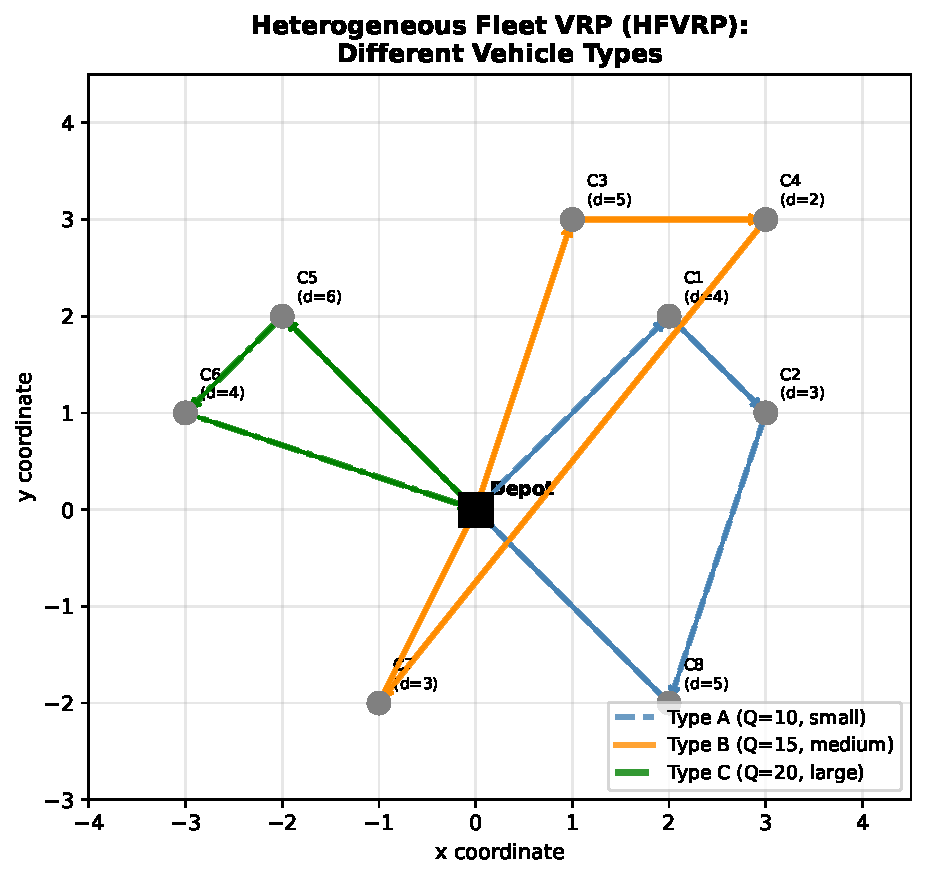
\includegraphics[width=0.72\textwidth]{hfvrp_routes.pdf}
\end{center}

In this example, three vehicle types serve 8 customers:
\begin{itemize}
  \item \textbf{Type A (Q=10, small)} --- serves customers $C1, C2, C8$
        (demands $4+3+5=12 > Q=10$, so the actual assignment must respect
        capacity; here drawn schematically).
  \item \textbf{Type B (Q=15, medium)} --- serves customers $C3, C4, C7$
        (demands $5+2+3=10 \leq 15$).
  \item \textbf{Type C (Q=20, large)} --- serves customers $C5, C6$
        (demands $6+4=10 \leq 20$).
\end{itemize}
The key insight is that the \emph{geographic clustering} of customers
interacts with \emph{vehicle capacity}: customers far from the depot benefit
from large vehicles to amortise the fixed cost over the long journey.

\end{frame}

%%--------------------------------------------------------------------
\begin{frame}[allowframebreaks]{HFVRP: Exact Methods}

\begin{block}{Set-Partitioning Formulation (Column Generation)}
  The standard exact approach for HFVRP uses a \textbf{set-partitioning}
  formulation where each column corresponds to a complete route for a specific
  vehicle type.  Let $\mathcal{R}_t$ be the set of all feasible routes for
  vehicle type $t$, and let $a_{ir}$ = 1 if customer $i$ appears in route
  $r$.  The formulation is:
  \[
    \min \sum_t \sum_{r \in \mathcal{R}_t} (f_t + \text{cost}_r) \cdot \lambda_r
  \]
  subject to:
  \[
    \sum_t \sum_{r \in \mathcal{R}_t} a_{ir} \lambda_r = 1 \quad \forall\, i
    \quad \text{(each customer covered exactly once)}
  \]
  \[
    \lambda_r \in \{0,1\} \quad \forall\, r
    \quad \text{(select or don't select each route)}
  \]
  where $\lambda_r$ (lambda, here $\lambda$ is read as ``lambda sub r'') is
  1 if route $r$ is selected and 0 otherwise, and $f_t$ is the fixed cost of
  the vehicle type used for route $r$.

  The LP relaxation is solved by Column Generation; the pricing sub-problem
  finds the route of minimum reduced cost for each vehicle type.
\end{block}

\begin{block}{Computational Results on Golden Instances}
  The benchmark instances due to \textbf{Golden et al.}\ have 20--483
  customers and up to 6 vehicle types.  Exact B\&P can solve the smaller
  instances (20--50 customers) optimally.  For larger instances, heuristics
  are required.
\end{block}

\end{frame}

%%--------------------------------------------------------------------
\begin{frame}[allowframebreaks]{HFVRP: Heuristics and Metaheuristics}

\begin{block}{Clarke-Wright Savings (Adapted)}
  The savings algorithm is adapted for HFVRP by choosing the cheapest vehicle
  type for each route.  After merging two routes, the algorithm selects the
  smallest vehicle type that has sufficient capacity for the combined route.
  This is efficient but may be suboptimal because it does not globally optimise
  vehicle-type assignments.
\end{block}

\begin{block}{Tabu Search (Gendreau, Laporte, Musaraganyi, Taillard)}
  The most influential metaheuristic for HFVRP was proposed by
  \textbf{Gendreau et al.}\ (1999).  Their Tabu Search uses:
  \begin{enumerate}
    \item \textbf{GENIUS insertion}: a powerful initial solution constructor
          that generalises nearest-neighbour insertion.
    \item \textbf{Move types}: single customer relocation, 2-opt, 3-opt,
          and vehicle type swap (change the vehicle assigned to an entire route).
    \item \textbf{Intensification}: restart from the best solution found and
          search more deeply.
    \item \textbf{Diversification}: when the search stagnates, randomly
          perturb the current solution.
  \end{enumerate}
  On the 12 Golden instances, this TS produces solutions within 2--4\% of the
  best known, with runtimes of seconds to minutes.
\end{block}

\framebreak

\begin{block}{Genetic Algorithm (Prins, 2009)}
  \textbf{Prins (2009)} proposed a GA with a chromosome encoding that
  simultaneously represents the permutation of customers and the vehicle-type
  assignment.  The crossover operator (LAX) preserves good partial routes
  from each parent.  A local search phase (2-opt, Or-opt) refines each
  offspring before it enters the population.  This hybrid GA is competitive
  with the best TS results on Golden instances.
\end{block}

\begin{block}{Simulated Annealing (Imran et al., 2009)}
  Simulated Annealing (SA) --- named after the annealing of metals, where
  slow cooling allows atoms to find a low-energy state --- accepts
  \emph{worse} solutions with a probability that decreases over time:
  \[
    P(\text{accept worse}) = \exp\!\bigl(-\Delta \text{cost} / T_{\text{current}}\bigr)
  \]
  where $T_{\text{current}}$ (the ``temperature'') starts high (accepting
  most moves) and gradually decreases (becoming more selective).  \textbf{Imran
  et al.}\ (2009) apply SA with a perturbation operator that swaps vehicle
  types between routes, achieving results competitive with Tabu Search on
  HFVRP benchmarks.
\end{block}

\begin{block}{Performance Comparison}
  \begin{center}
    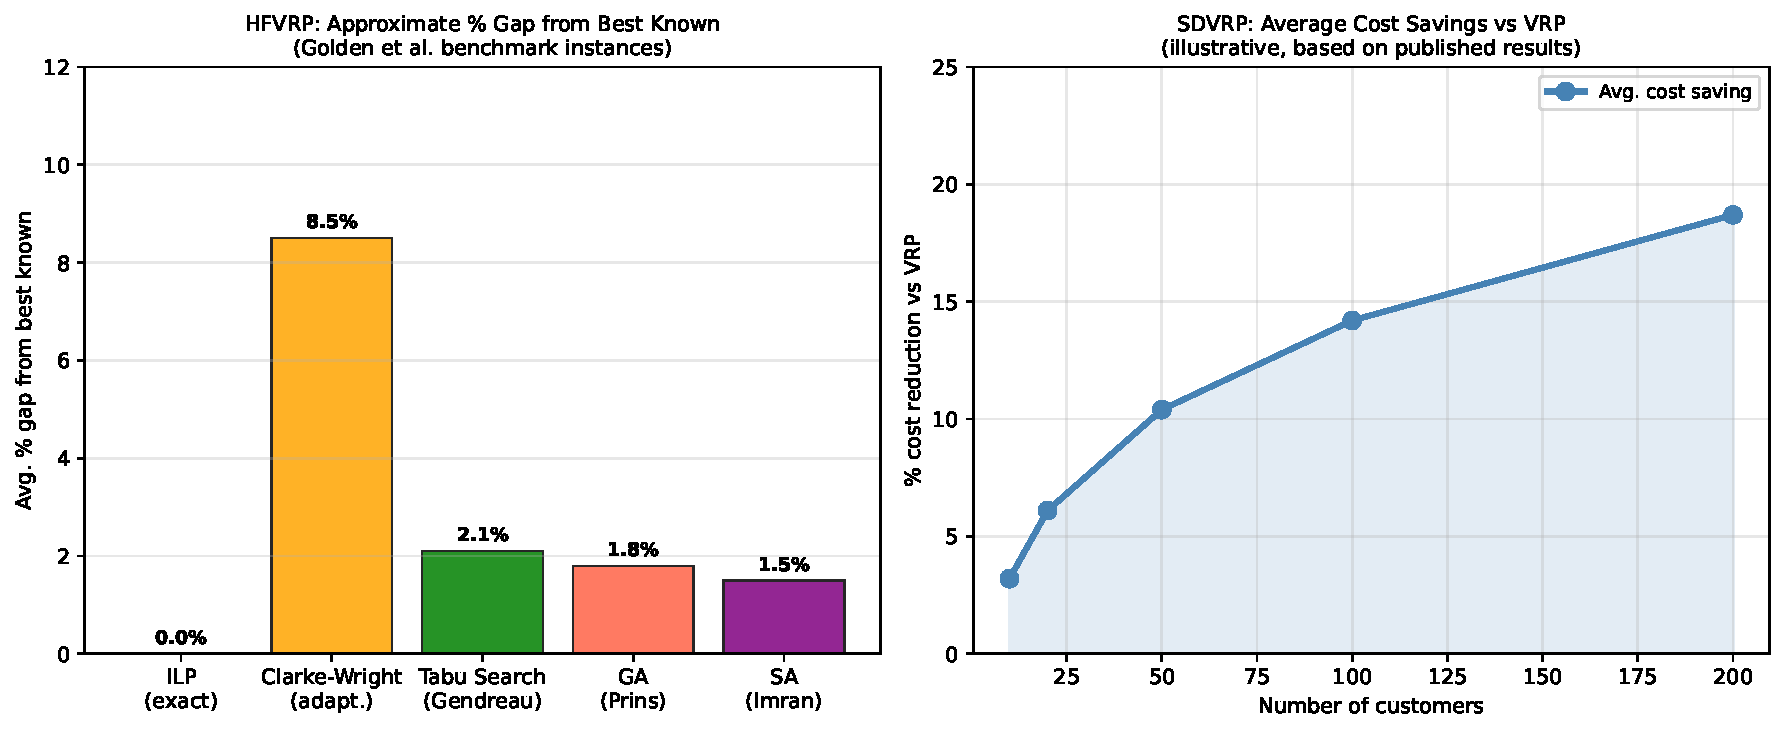
\includegraphics[width=0.70\textwidth]{algorithm_comparison.pdf}
  \end{center}
  The left panel shows approximate percentage gaps from the best known
  solutions on Golden instances.  Modern metaheuristics (TS, GA, SA) all
  achieve gaps of 1--3\%.
\end{block}

\end{frame}

%% ════════════════════════════════════════════════════════════════════════════
\section{9.4 Periodic Routing Problems (PVRP)}
%% ════════════════════════════════════════════════════════════════════════════

\begin{frame}[allowframebreaks]{9.4 PVRP: Problem Definition}

In many real logistics settings, routing is not a one-time decision but a
\emph{recurring} one.  A pharmaceutical distributor visits hospitals every
day; a bakery delivery service visits restaurants three times a week; a waste
collection company empties bins once or twice a week.  The
\textbf{Periodic Vehicle Routing Problem (PVRP)} captures this multi-period
planning structure.

\begin{block}{Formal Definition}
  The planning horizon consists of $T$ periods (days).  There are $n$
  customers; each customer $i$ has:
  \begin{itemize}
    \item $f_i \in \{1, 2, \ldots, T\}$ --- \textbf{visit frequency}: the
          number of times customer $i$ must be visited over the $T$-period
          horizon.
    \item A set $\mathcal{P}_i$ of \textbf{admissible visit patterns}: binary
          vectors $p = (p_1, \ldots, p_T)$ of length $T$ with exactly $f_i$
          ones, indicating on which days the customer is visited.  For example,
          with $T=5$ and $f_i=2$, a valid pattern is $(1,0,0,1,0)$ (Monday
          and Thursday).
    \item $d_i$ --- demand per visit (often assumed constant across visits).
  \end{itemize}
  The PVRP seeks to:
  \begin{enumerate}
    \item Assign an admissible visit pattern $p_i \in \mathcal{P}_i$ to each
          customer $i$.
    \item For each day $t = 1, \ldots, T$, build a set of routes serving all
          customers $i$ with $p_{it} = 1$.
    \item Minimise the total routing cost over all days, and optionally
          balance the daily workload.
  \end{enumerate}
\end{block}

\framebreak

\begin{block}{Why PVRP Is Harder than VRP}
  The PVRP is strictly harder than VRP for two reasons:
  \begin{enumerate}
    \item \textbf{Pattern assignment}: even before routing, we must decide
          \emph{which} $f_i$ days to visit each customer.  This is itself a
          combinatorial problem with $|\mathcal{P}_i|$ choices per customer.
          For $T=5$ and $f_i=2$, there are $\binom{5}{2}=10$ possible patterns.
    \item \textbf{Daily routing}: once patterns are assigned, we must solve a
          \emph{separate} VRP for each of the $T$ days --- so we are solving
          $T$ coupled VRPs simultaneously.
  \end{enumerate}
  The two sub-problems interact: a good pattern assignment leads to balanced
  daily demands that are easier to route efficiently.
\end{block}

\begin{center}
  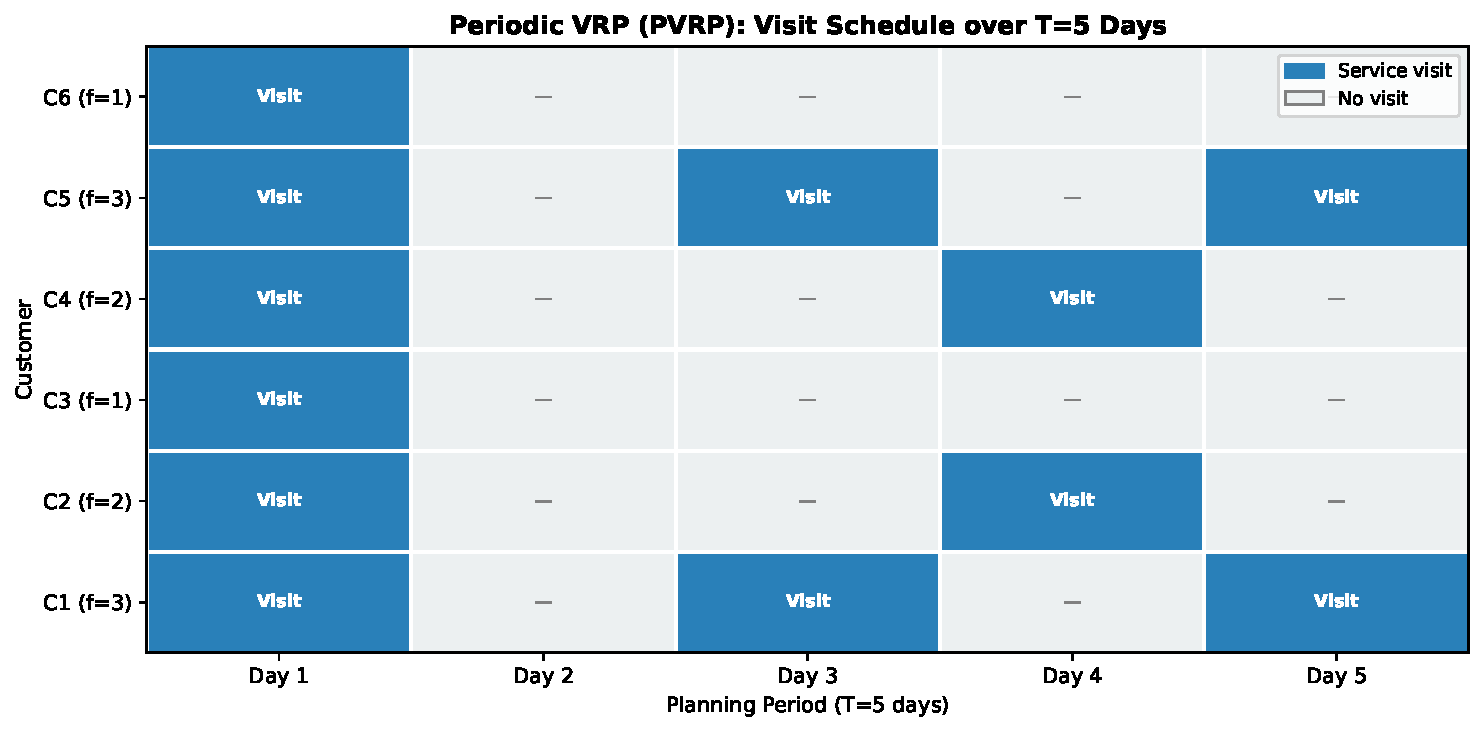
\includegraphics[width=0.85\textwidth]{pvrp_calendar.pdf}
\end{center}

\end{frame}

%%--------------------------------------------------------------------
\begin{frame}[allowframebreaks]{PVRP: Visit Patterns and Admissibility}

The set of admissible visit patterns for a customer with frequency $f_i$
over a $T$-period horizon consists of all binary vectors of length $T$
with exactly $f_i$ ones.  However, not all such vectors are \emph{practically
admissible}: for example, a customer requiring 3 visits per 5-day week
should not be visited three times on consecutive days if their inventory
can hold a week's worth of stock.  The admissible set $\mathcal{P}_i$ is
specified externally based on operational constraints.

\begin{center}
  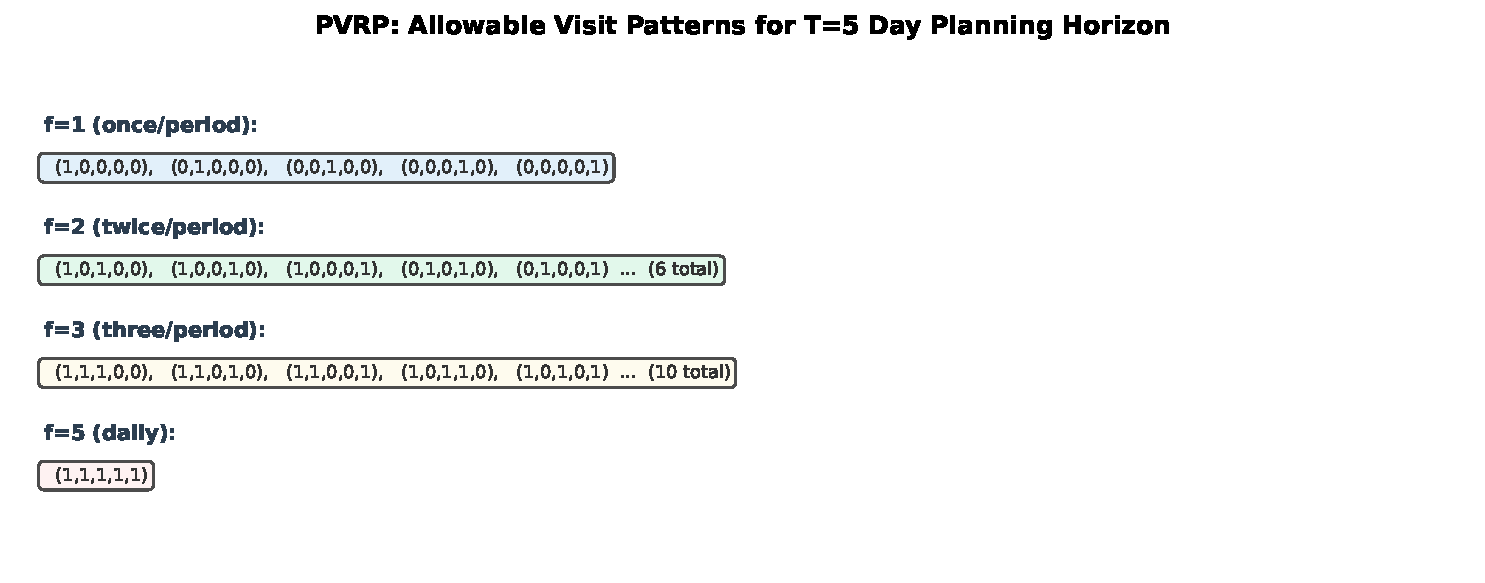
\includegraphics[width=0.80\textwidth]{pvrp_patterns.pdf}
\end{center}

\begin{block}{Standard Benchmark Patterns (Cordeau et al., 1997)}
  The most widely used PVRP benchmark (``p'' instances) uses $T=5$ and
  frequencies $f_i \in \{1,2,3,5\}$.  The admissible patterns are the
  standard patterns listed in the figure above.  A frequency-5 customer
  must be visited every day; a frequency-1 customer is visited once in
  any of the 5 days.  The assignment of patterns determines which
  customers appear in each day's routing problem.
\end{block}

\end{frame}

%%--------------------------------------------------------------------
\begin{frame}[allowframebreaks]{PVRP: Multi-Day Routes}

\begin{center}
  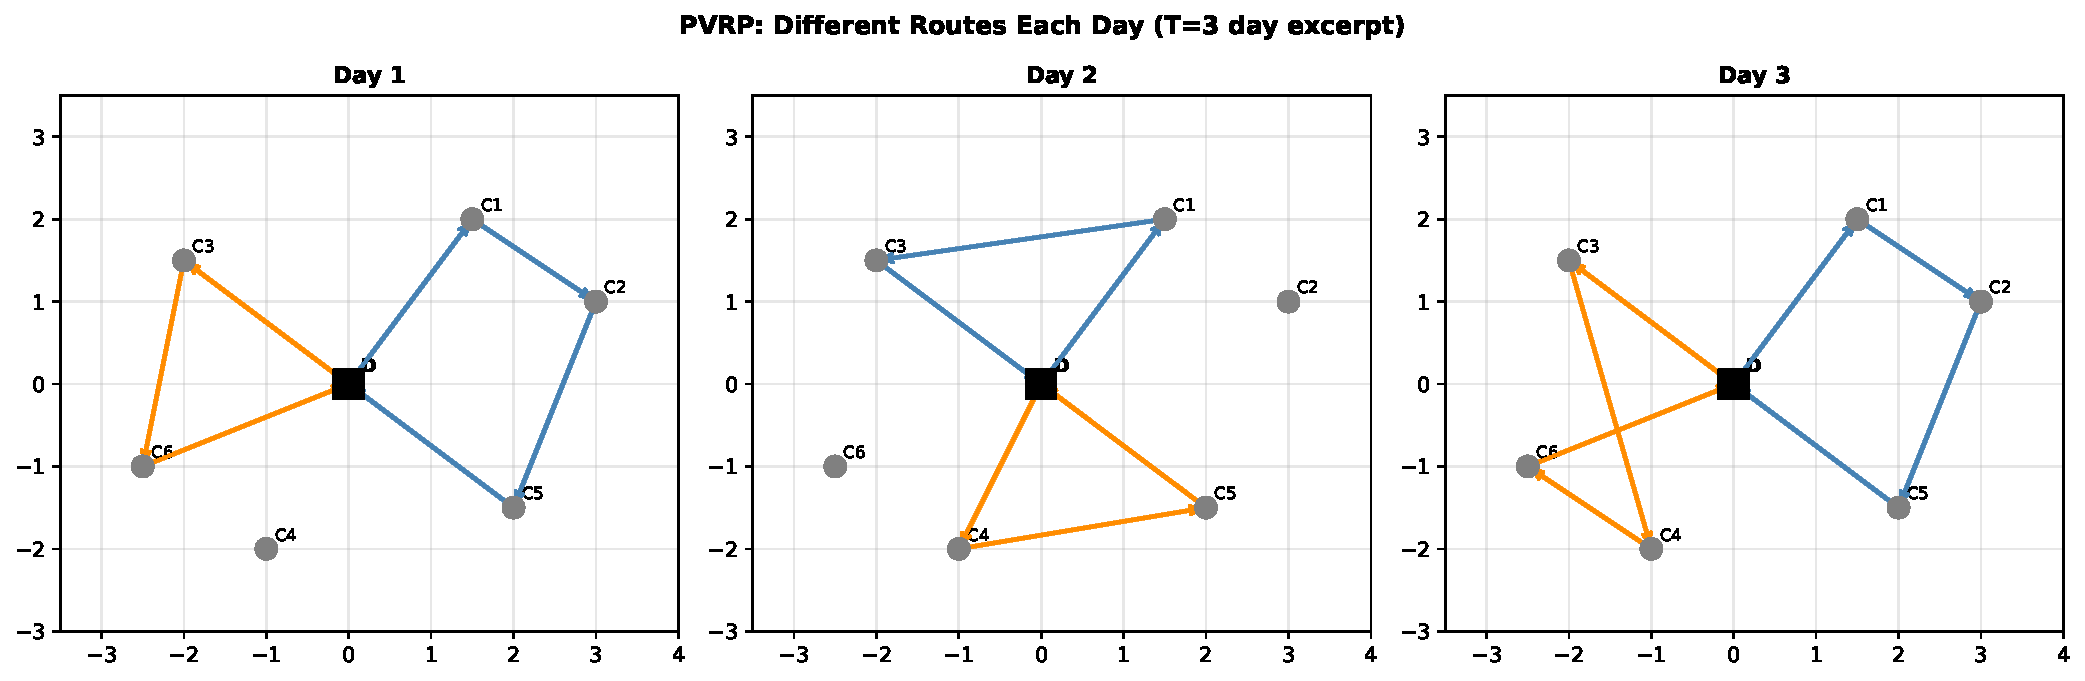
\includegraphics[width=0.90\textwidth]{pvrp_routes.pdf}
\end{center}

This figure shows how the same set of customers generates different daily
routes depending on their visit patterns.  On Day 1 (left), customers $C1,
C2, C5$ (high-frequency) and $C3, C6$ (who happen to have Day 1 in their
pattern) are visited.  On Day 2 (middle), a different subset is active.
The key point is that \emph{route structures change day to day}, and the
planner must design all $T$ days' routes simultaneously.

\begin{alertblock}{Workload Balancing}
  A secondary objective often included in PVRP is to make daily workloads as
  equal as possible.  If all high-demand customers are assigned to Monday,
  Monday's routing problem is large and expensive while other days are easy.
  Good pattern assignment distributes customers evenly over the week.
\end{alertblock}

\end{frame}

%%--------------------------------------------------------------------
\begin{frame}[allowframebreaks]{PVRP: The Standard (Benchmark) Formulation}

The standard PVRP formulation, introduced by \textbf{Cordeau, Gendreau, and
Laporte (1997)}, is a three-index integer program.

\begin{block}{Parameters and Variables}
  \begin{itemize}
    \item $n$ --- number of customers.
    \item $T$ --- number of periods (days) in the planning horizon.
    \item $m$ --- number of vehicles available per day.
    \item $Q$ --- vehicle capacity.
    \item $d_i$ --- demand of customer $i$ per visit.
    \item $c_{ij}$ --- travel cost between nodes $i$ and $j$.
    \item $\mathcal{P}_i$ --- set of admissible visit patterns for customer $i$.
    \item $z_{ip}$ --- equals 1 if pattern $p \in \mathcal{P}_i$ is selected
          for customer $i$, and 0 otherwise.  (``z sub i p'').
    \item $x_{ij}^{tk}$ --- equals 1 if vehicle $k$ traverses arc $(i,j)$ on
          day $t$.
  \end{itemize}
\end{block}

\begin{block}{Objective}
  \[
    \min \sum_{t=1}^{T} \sum_{k=1}^{m} \sum_{(i,j)\in A} c_{ij} x_{ij}^{tk}
  \]
  This sums travel cost over all days $t = 1,\ldots,T$, all vehicles
  $k = 1,\ldots,m$, and all arcs used.
\end{block}

\framebreak

\begin{block}{Key Constraints}
  \textbf{Pattern selection} (exactly one pattern per customer):
  \[
    \sum_{p \in \mathcal{P}_i} z_{ip} = 1 \quad \forall\, i \in \{1,\ldots,n\}
  \]

  \textbf{Linking patterns to daily routes}: if customer $i$ is assigned
  pattern $p$ with $p_t = 1$ (visited on day $t$), then $i$ must appear in
  day $t$'s routing:
  \[
    \sum_{j \in V} x_{ij}^{tk} = \sum_{p: p_t=1} z_{ip} \quad \forall\, i,\, \forall\, t
  \]

  \textbf{Daily VRP constraints}: for each day $t$, the routes $\{x^{tk}\}$
  form a feasible VRP solution: flow conservation, capacity, and sub-tour
  elimination.

  \textbf{Fleet size}: at most $m$ routes per day.
\end{block}

\end{frame}

%%--------------------------------------------------------------------
\begin{frame}[allowframebreaks]{PVRP: Exact and Heuristic Methods}

\begin{block}{Exact Methods}
  Exact methods for PVRP are based on Branch-and-Price.  The sub-problems
  decompose by day: for each day $t$, find routes of minimum reduced cost
  that cover the customers assigned to day $t$.  Cordeau, Gendreau, and
  Laporte (1997) applied this approach and solved the benchmark instances
  with up to 101 customers.  The LP lower bound is typically within 2--5\%
  of the optimum.
\end{block}

\begin{block}{Tabu Search (Cordeau et al., 1997 --- the definitive standard)}
  The most influential heuristic for PVRP is the \textbf{Unified Tabu Search}
  of Cordeau, Gendreau, and Laporte (1997), which handles multiple VRP
  variants under one framework.  The algorithm:
  \begin{enumerate}
    \item Starts with a greedy initial solution (insert customers into days
          that minimise cost increase, choosing among admissible patterns).
    \item At each iteration, moves a customer from one day's route to another
          (or changes their pattern assignment) by choosing the move with
          minimum cost increase (or maximum improvement).
    \item Forbids recently performed moves (tabu list) to prevent cycling.
    \item Applies penalties for constraint violations to allow temporary
          infeasibility and escape local optima.
  \end{enumerate}
  This TS routinely matches or improves the best known solutions on the
  standard PVRP benchmark.
\end{block}

\framebreak

\begin{block}{Metaheuristic Variants for PVRP}
  Several extensions of the standard TS have been proposed:
  \begin{itemize}
    \item \textbf{Granular Tabu Search} (Toth and Vigo, 2003): restricts
          moves to ``promising'' arcs (short arcs), dramatically reducing
          the neighbourhood size without sacrificing solution quality.  The
          \emph{granularity parameter} $\beta$ controls how many arcs are
          considered; typical values are $\beta = 1.5$--$3.0$.
    \item \textbf{Variable Neighbourhood Search (VNS)}: systematically
          explores different neighbourhood structures.  For PVRP, the
          neighbourhoods include pattern reassignment, within-day 2-opt,
          and cross-day customer relocation.
    \item \textbf{Evolutionary Local Search (ELS)}: combines a population
          of solutions with local search.  Each solution in the population
          is locally optimised; new solutions are generated by combining
          parts of high-quality solutions.
  \end{itemize}
\end{block}

\begin{block}{PVRP with Time Windows (PVRPTW)}
  A natural extension adds \emph{time windows} to the PVRP: each customer
  must be visited within a specified time interval on each visit day.  This
  makes the sub-problem for each day a \emph{VRPTW}, which is itself harder
  than VRP.  Heuristics for PVRPTW typically use the same TS framework but
  with a more complex feasibility check that includes time-window violations.
\end{block}

\end{frame}

%%--------------------------------------------------------------------
\begin{frame}[allowframebreaks]{PVRP: Other Variants}

\begin{block}{Multi-Depot PVRP (MDPVRP)}
  When there are multiple depots (each with its own fleet), the pattern
  assignment problem must also decide \emph{which depot} serves each customer
  on each visit day.  This adds a third dimension to the decision space.
  Valid approaches extend the PVRP TS by adding a depot-assignment operator:
  move a customer between depots as well as between days.
\end{block}

\begin{block}{PVRP with Service Time Dependence}
  In some applications, the service time or demand at a customer depends on
  the day of visit (e.g.\ supermarkets order more on Fridays before weekends).
  This time-dependent variant requires the pattern assignment to account for
  varying per-visit demands.
\end{block}

\begin{block}{PVRP as a Two-Phase Problem}
  A popular decomposition approach solves PVRP in two phases:
  \begin{enumerate}
    \item \textbf{Phase 1 (Pattern Assignment)}: assign a visit pattern to
          each customer, aiming to balance the daily customer load.  This
          can be solved approximately by a bin-packing or set-covering
          heuristic.
    \item \textbf{Phase 2 (Daily Routing)}: given the pattern assignments,
          solve $T$ independent VRPs (one per day) using a standard VRP
          solver.
  \end{enumerate}
  Two-phase methods are fast and easy to implement but may sacrifice quality
  because Phase 1 does not consider routing costs.  Integrated methods that
  solve both phases simultaneously generally outperform them.
\end{block}

\end{frame}

%% ════════════════════════════════════════════════════════════════════════════
\section{9.5 VRP with Split Deliveries (SDVRP)}
%% ════════════════════════════════════════════════════════════════════════════

\begin{frame}[allowframebreaks]{9.5 SDVRP: Problem Definition}

In the classical VRP, each customer must be served by \emph{exactly one
vehicle}.  This constraint can be wasteful: if a customer requires 9 units
and the vehicle capacity is 10, then that vehicle is nearly full but carries
only one customer's goods.  The \textbf{Split Delivery VRP (SDVRP)} relaxes
this constraint, allowing a customer's demand to be split across multiple
vehicles.

\begin{block}{Formal Definition}
  We have $n$ customers, each with demand $d_i > 0$, and $m$ vehicles each
  with capacity $Q$.  The SDVRP allows customer $i$ to be visited by multiple
  vehicles, receiving a partial delivery $d_i^v > 0$ from vehicle $v$ (where
  $v$ ranges over all vehicles that visit $i$), as long as the total delivery
  equals the full demand:
  \[
    \sum_{v: v \text{ visits } i} d_i^v = d_i \quad \forall\, i.
  \]
  The \textbf{number of times} a customer is visited (split deliveries) is
  unrestricted (in principle), but in practice most algorithms limit splits
  to avoid excessive customer inconvenience.
\end{block}

\begin{block}{Intuition: Why Splitting Helps}
  Imagine two customers each needing 8 units, with $Q = 10$.  Without
  splitting: 2 separate routes needed (8 units each, capacity wasted).  With
  splitting: one vehicle carries 8 for customer 1 and 2 for customer 2
  (full load); another vehicle carries 6 for customer 2 (also full).  We
  have saved one depot-return trip at the cost of visiting customer 2 twice.
\end{block}

\end{frame}

%%--------------------------------------------------------------------
\begin{frame}[allowframebreaks]{SDVRP: Split vs. No-Split Comparison}

\begin{center}
  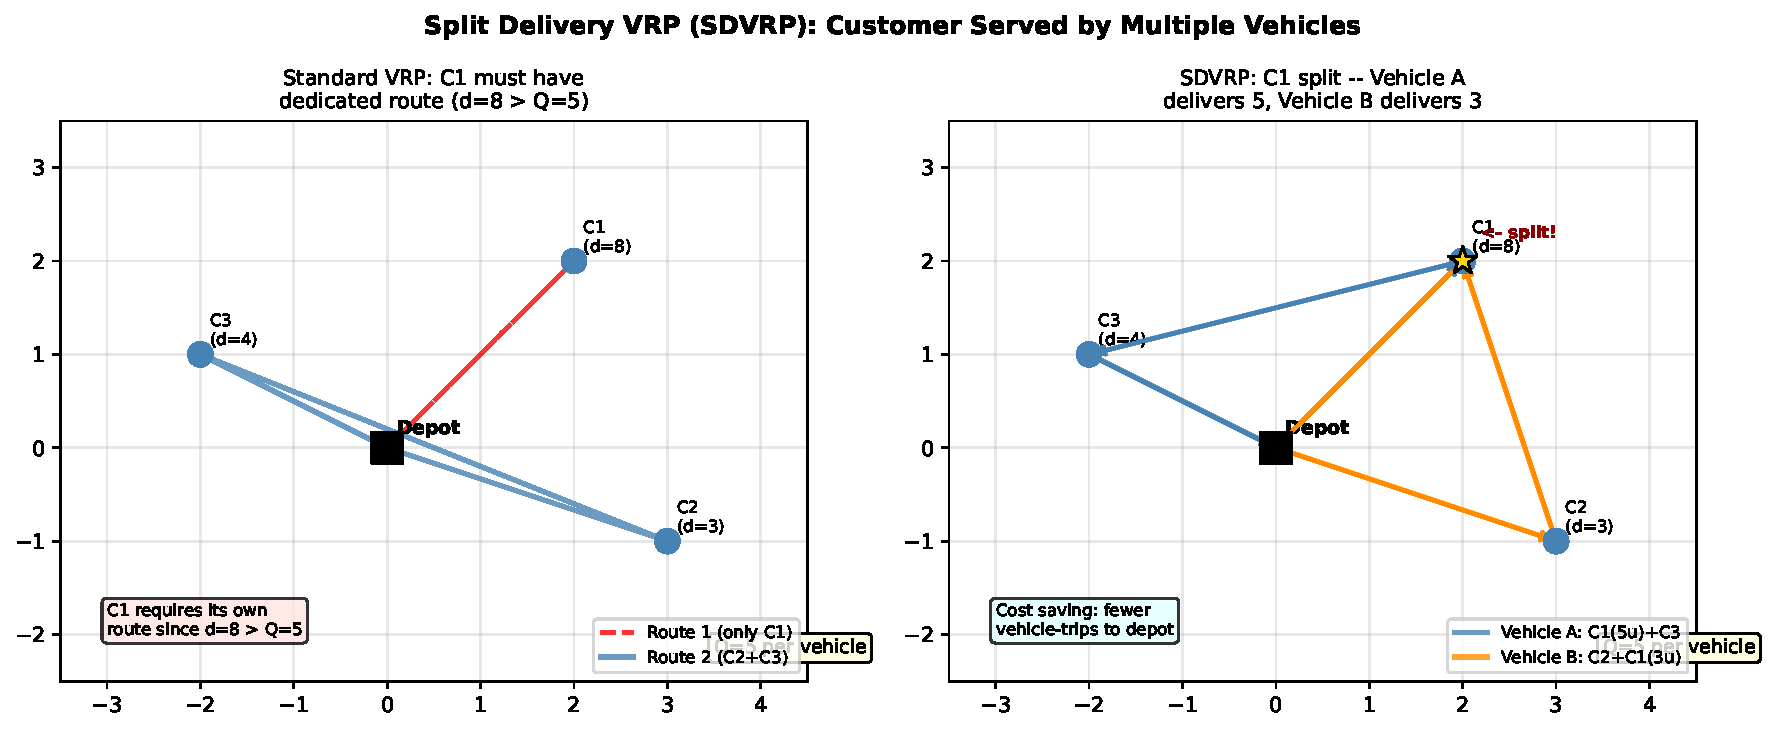
\includegraphics[width=0.90\textwidth]{sdvrp_split.pdf}
\end{center}

The left panel shows the standard VRP where customer $C1$ (demand 8 $> Q=5$)
must have a dedicated route.  The right panel shows the SDVRP where $C1$ is
split: Vehicle A delivers 5 units to $C1$ on one trip, Vehicle B delivers the
remaining 3 units on another trip while also serving $C2$ and $C3$.  The
total number of routes is reduced from 2 to 2 here, but the key saving is
that Vehicle A can now also serve $C3$ on its trip --- reducing total
distance.

\begin{alertblock}{The Fundamental Trade-Off in SDVRP}
  Splitting a customer reduces the number of routes (fewer vehicles needed)
  but may increase the number of visits to some customers, which is
  inconvenient for the customer and increases operational complexity.  The
  SDVRP finds the sweet spot: split only when the distance/cost saving
  justifies the extra visit.
\end{alertblock}

\end{frame}

%%--------------------------------------------------------------------
\begin{frame}[allowframebreaks]{SDVRP: Mathematical Formulation and Basic Variant}

The SDVRP was first studied by \textbf{Dror and Trudeau (1989, 1990)}.
They showed that the problem on a tree network can be solved in polynomial
time, but the general (Euclidean or graph) case is NP-hard.

\begin{block}{Basic SDVRP Formulation}
  Let $x_{ij}^v \in \{0,1\}$ indicate whether vehicle $v$ traverses arc
  $(i,j)$, and let $q_i^v \geq 0$ be the amount delivered to customer $i$
  by vehicle $v$.  Then:
  \[
    \min \sum_v \sum_{(i,j)\in A} c_{ij} x_{ij}^v
  \]
  subject to:
  \[
    \sum_v q_i^v = d_i \quad \forall\, i
    \qquad \text{(full demand satisfied)}
  \]
  \[
    q_i^v \leq d_i \cdot \sum_{j \in V} x_{ij}^v \quad \forall\, i, v
    \qquad \text{(delivery only if vehicle visits)}
  \]
  \[
    \sum_i q_i^v \leq Q \quad \forall\, v
    \qquad \text{(capacity per vehicle)}
  \]
  Flow conservation and sub-tour elimination constraints complete the model.
\end{block}

\framebreak

\begin{block}{Lower Bound: Number of Vehicles Required}
  A fundamental property of the SDVRP is that the minimum number of vehicles
  required to serve all customers is:
  \[
    m^* = \left\lceil \frac{\sum_{i=1}^n d_i}{Q} \right\rceil
  \]
  where $\lceil \cdot \rceil$ (the ceiling function) rounds up to the nearest
  integer.  Here $\sum_{i=1}^n d_i$ is the \textbf{total demand} (sum of
  all customers' demands) and $Q$ is the vehicle capacity.  This bound
  follows from the fact that with split deliveries, we can \emph{always}
  fill each vehicle completely (except possibly the last one), so the
  minimum number of vehicle-loads needed is exactly $\lceil D/Q \rceil$
  where $D = \sum_i d_i$.

  \medskip
  In contrast, without splitting, bin-packing constraints may force us to
  use \emph{more} than $\lceil D/Q \rceil$ vehicles because demands may not
  pack perfectly.
\end{block}

\begin{exampleblock}{Worked Example: Savings from Splitting}
  Five customers with demands $[8, 7, 6, 9, 5]$, total $D = 35$, capacity
  $Q = 10$.
  \begin{itemize}
    \item \textbf{Lower bound} (split allowed): $\lceil 35/10 \rceil = 4$
          vehicles minimum.
    \item \textbf{Without splitting} (bin packing): demands $[9,8,7,6,5]$
          sorted descending.  First route: 9 only (room for 1 more: $9+8 > 10$
          so 9 alone); Second: 8 alone; Third: $7+3 \leq 10$ but no customer
          with demand 3 exists; and so on.  Result: 5 vehicles needed.
    \item \textbf{With splitting}: 4 vehicles (saving 1 vehicle trip).
  \end{itemize}
\end{exampleblock}

\end{frame}

%%--------------------------------------------------------------------
\begin{frame}[allowframebreaks]{SDVRP: Theoretical Properties}

Dror and Trudeau (1989, 1990) proved several key properties that guide the
design of algorithms for the SDVRP.

\begin{block}{Property 1: Optimal Split Structure}
  In an optimal SDVRP solution, if a customer $i$ is visited by more than
  one vehicle, it is visited at most twice (under certain triangle-inequality
  conditions on the distances).  This is a remarkable result: even though
  in principle a customer could be visited many times, twice is almost always
  sufficient in practice.
\end{block}

\begin{block}{Property 2: Maximum Savings from Splitting}
  The cost ratio between the optimal VRP solution (no split) and the optimal
  SDVRP solution (split allowed) is bounded:
  \[
    \frac{\text{VRP}^*}{\text{SDVRP}^*} \leq 1 + \frac{1}{2\lceil Q/d_{\min}\rceil - 1}
  \]
  where $d_{\min}$ is the smallest customer demand.  Here $Q/d_{\min}$ is
  the ratio of vehicle capacity to the smallest demand; $\lceil Q/d_{\min} \rceil$
  is the maximum number of customers a vehicle can carry if all have minimum
  demand.  When this number is large (small demands relative to capacity),
  the bound approaches 1 --- splitting gives little benefit because vehicles
  are already nearly full.  When demands are close to $Q$, splitting can
  give savings of up to 50\%.
\end{block}

\begin{center}
  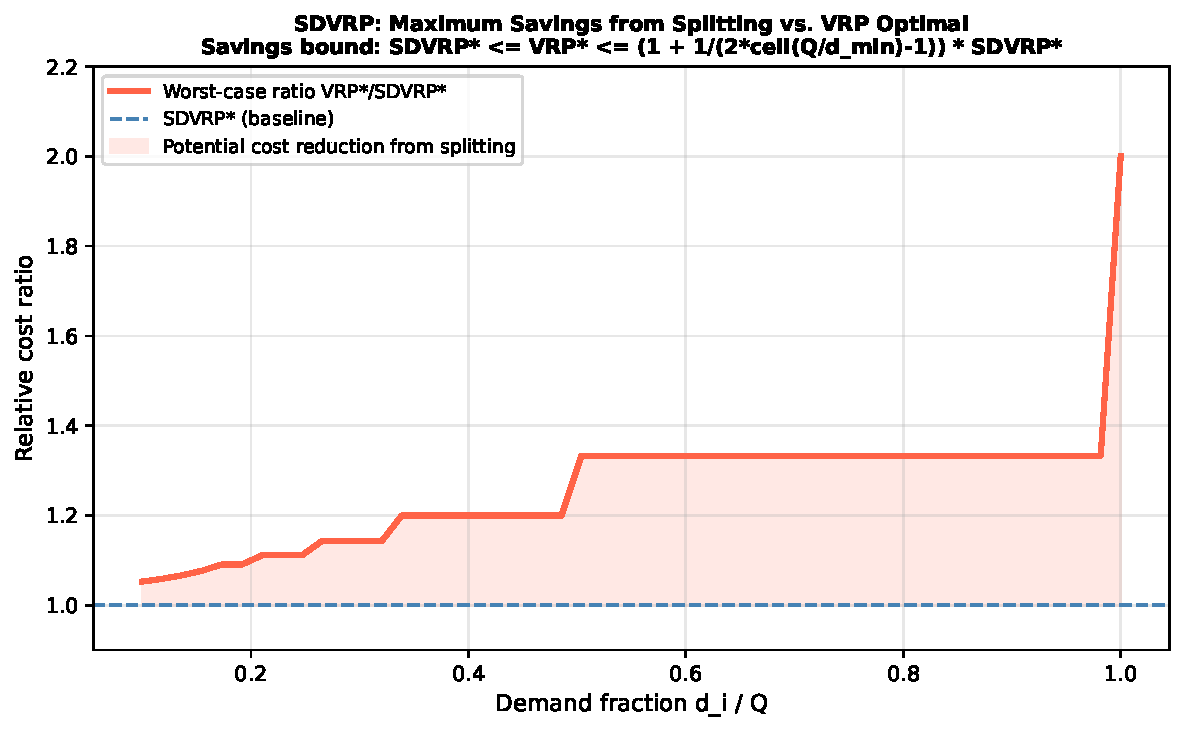
\includegraphics[width=0.60\textwidth]{sdvrp_savings_bound.pdf}
\end{center}

\end{frame}

%%--------------------------------------------------------------------
\begin{frame}[allowframebreaks]{SDVRP: Exact and Heuristic Methods}

\begin{block}{Exact Methods (Archetti, Speranza, Hertz)}
  Exact algorithms for the SDVRP use Branch-and-Price.  The pricing
  sub-problem is a \emph{shortest path problem with resource constraints}:
  find a minimum-cost route (path from depot through a subset of customers
  back to depot) that respects capacity, where customers may be visited
  partially (split loads).  This sub-problem is NP-hard in general, but
  efficient label-setting algorithms handle it in practice.

  \medskip
  \textbf{Archetti, Speranza, and Hertz (2006)} developed a B\&P that can
  solve instances with up to 100 customers to optimality.  The key
  observation is that in the LP relaxation of the set-partitioning master
  problem, customers with demand $d_i > Q/2$ \emph{must} be split (they
  cannot fit in a single vehicle with anyone else), so these splits are
  pre-processed.
\end{block}

\begin{block}{Heuristics: Nearest-Neighbour and Insertion}
  Simple constructive heuristics for SDVRP work as follows:
  \begin{enumerate}
    \item Initialise each vehicle at the depot with a full load of $Q$ units.
    \item At each step, the current vehicle visits the nearest unserved
          customer (or the nearest customer with remaining undelivered demand).
    \item If the vehicle can fully serve the customer, do so.  If not (demand
          exceeds remaining capacity), deliver the remaining capacity as a
          partial delivery, mark the customer as partially served, and return
          to depot.
    \item Continue until all customers are fully served.
  \end{enumerate}
  This greedy approach is fast but may give solutions 10--20\% above optimal.
\end{block}

\framebreak

\begin{block}{Tabu Search for SDVRP (Archetti, Hertz, Speranza, 2006)}
  The most effective published TS for SDVRP uses these neighbourhoods:
  \begin{itemize}
    \item \textbf{Split/unsplit}: take a partially-served customer and either
          merge the two partial deliveries into one (unsplit) or further split
          an existing single delivery (create a new partial delivery on another
          vehicle).
    \item \textbf{Customer relocation}: move a (partial) delivery from one
          route to another.
    \item \textbf{2-opt within a route}: reverse a segment of a route, check
          that capacity is not violated.
    \item \textbf{Interchange}: swap deliveries between two routes.
  \end{itemize}
  On benchmark instances, this TS produces solutions within 0.5--2\% of the
  best known in seconds.
\end{block}

\begin{block}{The SDVRP with Time Windows (SDVRPTW)}
  Combining split deliveries with time windows is particularly challenging:
  a split customer must be visited at \emph{different times} by different
  vehicles, so the time windows must be consistent across all visits.  The
  B\&P approach extends to SDVRPTW with additional time-window constraints
  in the pricing sub-problem.
\end{block}

\end{frame}

%%--------------------------------------------------------------------
\begin{frame}[allowframebreaks]{SDVRP: Variants and Extensions}

\begin{center}
  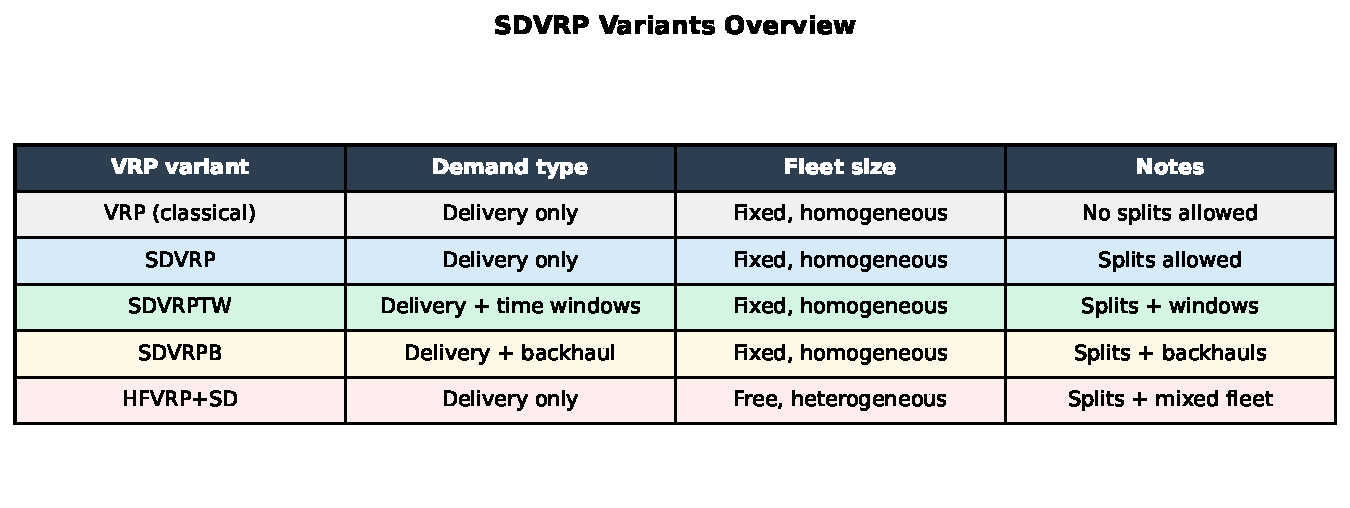
\includegraphics[width=0.75\textwidth]{sdvrp_table.pdf}
\end{center}

\begin{block}{SDVRP with Backhauls (SDVRPB)}
  When split deliveries are combined with backhaul customers, the problem
  becomes significantly more complex.  Now linehaul customers may have their
  demand split across multiple vehicles, and backhaul pickups must still
  come after all linehaul deliveries on each route.  Heuristics adapt the
  standard SDVRP operators by checking the precedence constraint after every
  move.
\end{block}

\begin{block}{Savings from Splitting: Empirical Observations}
  Empirical studies on real-world instances suggest:
  \begin{itemize}
    \item For instances where $d_i \leq Q/3$ for all customers (small demands
          relative to capacity), splitting gives negligible savings.
    \item For instances where $d_i \approx Q/2$ for many customers (medium
          demands), savings of 5--15\% in total distance are typical.
    \item For instances where some customers have $d_i > Q$ (demands larger
          than capacity), splitting is \emph{mandatory}: the customer
          \emph{must} be split.
  \end{itemize}
\end{block}

\end{frame}

%% ════════════════════════════════════════════════════════════════════════════
\section{9.6 Python Implementations}
%% ════════════════════════════════════════════════════════════════════════════

\begin{frame}[fragile]{Python: VRPB Savings Algorithm}

The following Python code implements the Clarke-Wright savings algorithm
adapted for VRPB.  It starts with individual routes, computes savings for
all linehaul pairs, merges the best feasible pair, then does the same for
backhauls, and finally attempts to join linehaul and backhaul routes when
capacity allows.

\begin{lstlisting}
import numpy as np
from itertools import combinations

def vrpb_savings(depot, linehauls, backhauls, demands, Q):
    """
    Clarke-Wright savings algorithm for VRPB.
    depot : (x,y) tuple
    linehauls : dict {name: (x,y)}
    backhauls  : dict {name: (x,y)}
    demands    : dict {name: demand}
    Q          : vehicle capacity
    Returns list of routes, each a list of customer names.
    """
    all_c = {**linehauls, **backhauls}
    # Distance helper
    def dist(a, b):
        return np.hypot(a[0]-b[0], a[1]-b[1])

    # Initial solution: each customer alone
    routes = {c: [c] for c in all_c}
    loads  = {c: demands[c] for c in all_c}

    # Compute all savings s(i,j) = d(depot,i) + d(depot,j) - d(i,j)
    # Only merge same type (linehaul-linehaul OR backhaul-backhaul first)
    savings = []
    all_names = list(all_c.keys())
    for i, j in combinations(all_names, 2):
        s = dist(depot, all_c[i]) + dist(depot, all_c[j]) - dist(all_c[i], all_c[j])
        savings.append((s, i, j))
    savings.sort(reverse=True)  # best savings first

    # Greedy merge
    def can_merge(r1_name, r2_name):
        r1 = routes[r1_name]; r2 = routes[r2_name]
        # Check: must not mix L after B (linehaul must come first)
        combined = r1 + r2
        seen_backhaul = False
        for c in combined:
            if c in backhauls:
                seen_backhaul = True
            elif seen_backhaul:  # linehaul after backhaul: infeasible
                return False
        # Check capacity
        if loads[r1_name] + loads[r2_name] > Q:
            return False
        return True

    for s, i, j in savings:
        # Find route owners
        ri = next((k for k, v in routes.items() if i in v), None)
        rj = next((k for k, v in routes.items() if j in v), None)
        if ri is None or rj is None or ri == rj:
            continue  # already merged or same route
        if can_merge(ri, rj):
            routes[ri] = routes[ri] + routes[rj]
            loads[ri] += loads[rj]
            del routes[rj]; del loads[rj]

    return list(routes.values())

# Example usage
depot = (0, 0)
linehauls = {'L1': (3, 2), 'L2': (2, 4)}
backhauls  = {'B1': (-2, 1), 'B2': (-3, -1)}
demands    = {'L1': 4, 'L2': 5, 'B1': 3, 'B2': 4}
Q = 10
result = vrpb_savings(depot, linehauls, backhauls, demands, Q)
print("Routes:", result)
\end{lstlisting}

\end{frame}

%%--------------------------------------------------------------------
\begin{frame}[fragile]{Python: SDVRP Minimum Vehicles and Greedy Split}

This code computes the theoretical minimum number of vehicles for the SDVRP
and implements a simple greedy split delivery heuristic.

\begin{lstlisting}
import math

def sdvrp_min_vehicles(demands, Q):
    """
    Compute the lower bound on number of vehicles needed with split deliveries.
    demands : list of customer demands
    Q       : vehicle capacity
    """
    total_demand = sum(demands)
    return math.ceil(total_demand / Q)

def sdvrp_greedy(customers, demands, Q):
    """
    Greedy split delivery heuristic.
    customers : list of (x,y) customer positions (index = customer ID)
    demands   : list of demands (same indexing)
    Q         : vehicle capacity
    Returns list of vehicle routes: each route is list of (customer_id, qty_delivered).
    """
    import numpy as np
    remaining = list(demands)  # remaining demand for each customer
    n = len(customers)
    routes = []

    while any(r > 0 for r in remaining):
        route = []
        load = Q
        # Current position starts at depot (0,0)
        pos = np.array([0.0, 0.0])

        while load > 0:
            # Find nearest customer with remaining demand
            best_i, best_d = -1, float('inf')
            for i in range(n):
                if remaining[i] > 0:
                    d = np.linalg.norm(np.array(customers[i]) - pos)
                    if d < best_d:
                        best_d, best_i = d, i
            if best_i == -1:
                break  # all served
            # Deliver as much as possible
            qty = min(remaining[best_i], load)
            route.append((best_i, qty))
            remaining[best_i] -= qty
            load -= qty
            pos = np.array(customers[best_i])

        routes.append(route)

    return routes

# Example
customers = [(2,2), (3,-1), (-2,1), (-3,-1), (1,-3)]
demands   = [8, 7, 6, 9, 5]
Q = 10

min_v = sdvrp_min_vehicles(demands, Q)
print(f"Minimum vehicles needed: {min_v}")  # = ceil(35/10) = 4
routes = sdvrp_greedy(customers, demands, Q)
print(f"Greedy routes: {len(routes)} vehicles used")
for i, r in enumerate(routes):
    print(f"  Vehicle {i+1}: {r}")
\end{lstlisting}

\end{frame}

%%--------------------------------------------------------------------
\begin{frame}[fragile]{Python: PVRP Pattern Assignment}

The following code demonstrates pattern assignment for the PVRP: given
customer frequencies and admissible patterns, it assigns patterns to balance
the daily workload (number of customers per day).

\begin{lstlisting}
from itertools import combinations

def generate_patterns(T, f):
    """
    Generate all binary vectors of length T with exactly f ones.
    T : planning horizon (number of days)
    f : visit frequency
    Returns list of tuples, each a binary pattern.
    """
    return [tuple(1 if i in combo else 0 for i in range(T))
            for combo in combinations(range(T), f)]

def pvrp_balance_assignment(n_customers, frequencies, T):
    """
    Assign visit patterns to balance daily customer load.
    n_customers : number of customers
    frequencies : list of visit frequencies (one per customer)
    T           : number of days in planning horizon
    Returns list of assigned patterns (one per customer).
    """
    # Daily load tracker
    daily_load = [0] * T
    assigned = []

    for i, f in enumerate(frequencies):
        patterns = generate_patterns(T, f)
        # Choose pattern that minimises the maximum daily load after assignment
        best_pat, best_max = None, float('inf')
        for pat in patterns:
            test_load = [daily_load[d] + pat[d] for d in range(T)]
            if max(test_load) < best_max:
                best_max = max(test_load)
                best_pat = pat
        assigned.append(best_pat)
        daily_load = [daily_load[d] + best_pat[d] for d in range(T)]

    return assigned, daily_load

# Example: 6 customers, T=5 days
frequencies = [3, 2, 1, 2, 3, 1]
T = 5
patterns, daily_load = pvrp_balance_assignment(6, frequencies, T)
print("Assigned patterns:")
days = ['Mon','Tue','Wed','Thu','Fri']
for i, (f, p) in enumerate(zip(frequencies, patterns)):
    visit_days = [days[d] for d in range(T) if p[d]]
    print(f"  Customer {i+1} (f={f}): visits {visit_days}")
print(f"\nDaily customer counts: {dict(zip(days, daily_load))}")
\end{lstlisting}

\end{frame}

%% ════════════════════════════════════════════════════════════════════════════
\section{9.7 Conclusions and Future Research}
%% ════════════════════════════════════════════════════════════════════════════

\begin{frame}[allowframebreaks]{9.7 Conclusions and Future Research Directions}

This chapter has surveyed four important variants of the VRP, each capturing
a different real-world feature that the classical model cannot handle.

\begin{block}{Summary: What Each Variant Adds}
  \begin{center}
  \renewcommand{\arraystretch}{1.4}
  \begin{tabular}{>{\bfseries}p{1.8cm}p{3.5cm}p{2.8cm}p{3.2cm}}
    \toprule
    Variant & Real-World Motivation & Key Constraint & Best Method (large $n$) \\
    \midrule
    VRPB  & Delivery + collection
           & Linehaul before backhaul
           & Tabu Search, ALNS \\
    HFVRP & Mixed fleet (trucks of different sizes)
           & Choose vehicle type per route
           & Tabu Search, GA \\
    PVRP  & Weekly delivery schedules
           & Visit frequency + pattern assignment
           & Unified Tabu Search \\
    SDVRP & Large demands, bin-packing waste
           & Full demand split across vehicles
           & B\&P (exact), TS (heuristic) \\
    \bottomrule
  \end{tabular}
  \end{center}
\end{block}

\framebreak

\begin{block}{Open Research Questions}
  \begin{enumerate}
    \item \textbf{Exact algorithms for large instances}: current exact methods
          (B\&P) top out at $\approx100$ customers for all four variants.
          Advances in cut-generation, branch-and-cut-and-price, and
          decomposition are needed for larger instances.
    \item \textbf{Hybrid variants}: all four variants can be combined (e.g.\
          PVRP with heterogeneous fleet and backhauls).  These combinations
          are increasingly common in practice but barely studied theoretically.
    \item \textbf{Stochastic and dynamic extensions}: demands may be uncertain,
          customers may cancel, or new orders may arrive mid-route.  Robust
          and online versions of VRPB, HFVRP, PVRP, and SDVRP are active
          research areas.
    \item \textbf{Electric vehicles in HFVRP}: as fleets transition to electric
          vehicles (EVs), capacity constraints are joined by battery range
          constraints and charging decisions --- a new dimension for the
          heterogeneous fleet problem.
    \item \textbf{Machine learning for pattern selection (PVRP)}: pattern
          assignment in PVRP is a combinatorial assignment problem that may
          benefit from reinforcement learning approaches that learn good
          assignment policies from historical routing data.
  \end{enumerate}
\end{block}

\framebreak

\begin{alertblock}{Take-Away Message}
  The four variants studied in this chapter --- VRPB, HFVRP, PVRP, SDVRP ---
  are not academic curiosities.  They arise directly from the physical and
  operational constraints of real distribution systems.  Understanding the
  structure of each variant --- its key constraint, its lower bounds, and the
  algorithms that exploit its structure --- equips a practitioner to design
  efficient routing systems and to recognise which off-the-shelf VRP solver
  (if any) is appropriate for a given application.
\end{alertblock}

\end{frame}

%% ════════════════════════════════════════════════════════════════════════════
\section{Appendix: Additional Figures}
%% ════════════════════════════════════════════════════════════════════════════

\begin{frame}[allowframebreaks]{Appendix: VRPB Formulation Summary}

\begin{center}
  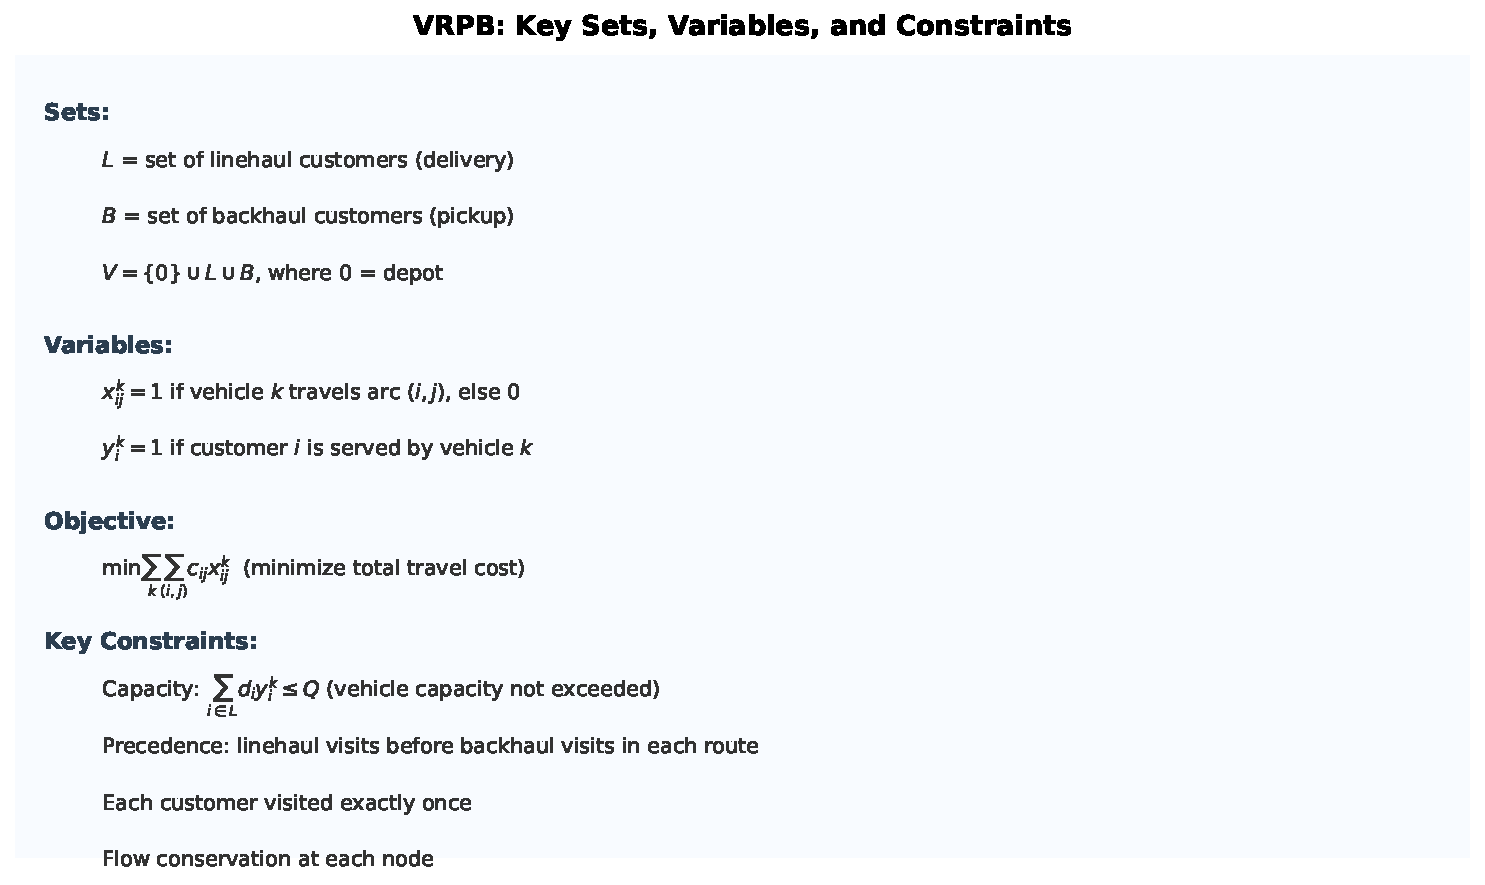
\includegraphics[width=0.85\textwidth]{vrpb_formulation.pdf}
\end{center}

This figure summarises the key sets, variables, objective function, and
constraints of the VRPB ILP formulation.  The precedence constraint is
enforced by forbidding any arc from a backhaul node to a linehaul node.
The capacity constraints (using MTZ variables $u_i$) simultaneously eliminate
sub-tours and enforce vehicle loading limits.

\end{frame}

%%--------------------------------------------------------------------
\begin{frame}[allowframebreaks]{Appendix: SDVRP Savings Bound Illustration}

\begin{center}
  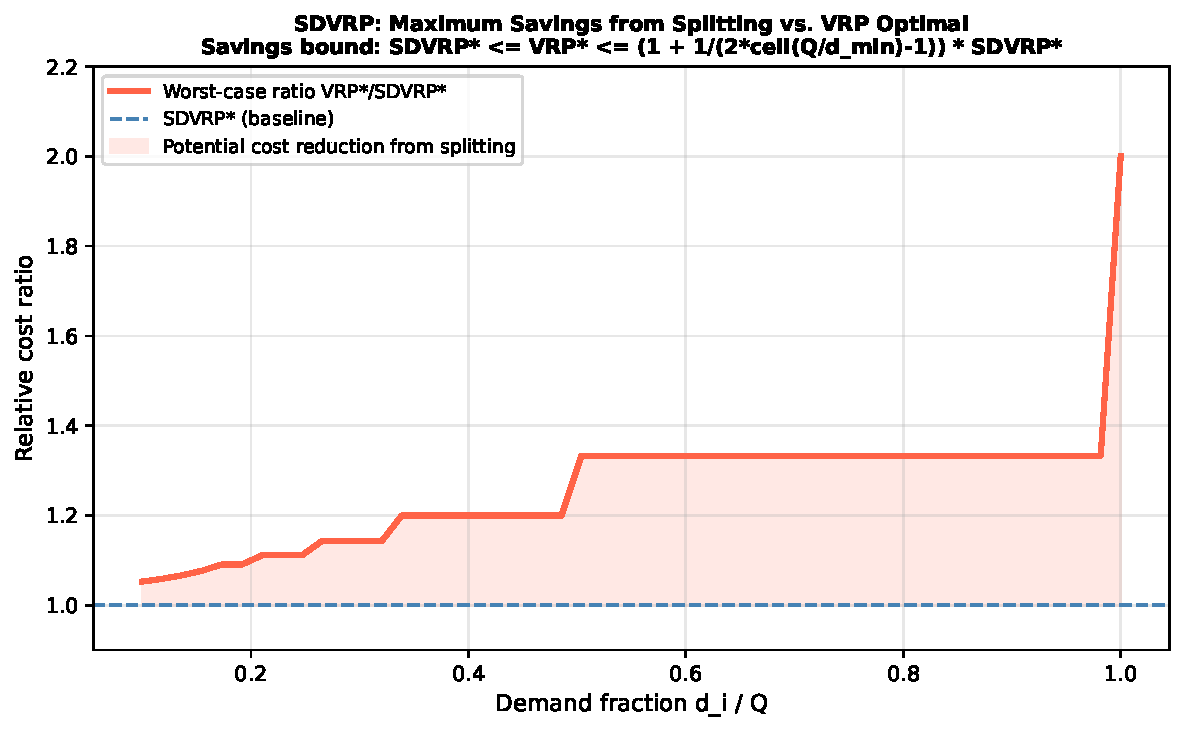
\includegraphics[width=0.72\textwidth]{sdvrp_savings_bound.pdf}
\end{center}

This plot illustrates the theoretical bound on the ratio $\text{VRP}^* /
\text{SDVRP}^*$ as a function of the demand fraction $d_i/Q$ (the ratio
of a customer's demand to the vehicle capacity).  When demands are small
relative to capacity (left side of the plot), the bound approaches 1 ---
splitting gives no benefit.  When demands approach the full capacity
(right side), the bound can be as large as 2 --- standard VRP can cost up
to twice as much as the optimal split-delivery solution.  The shaded region
represents the potential cost reduction available through split deliveries.

\end{frame}

%%--------------------------------------------------------------------
\begin{frame}[allowframebreaks]{Appendix: VRPB Three Variants Side by Side}

\begin{center}
  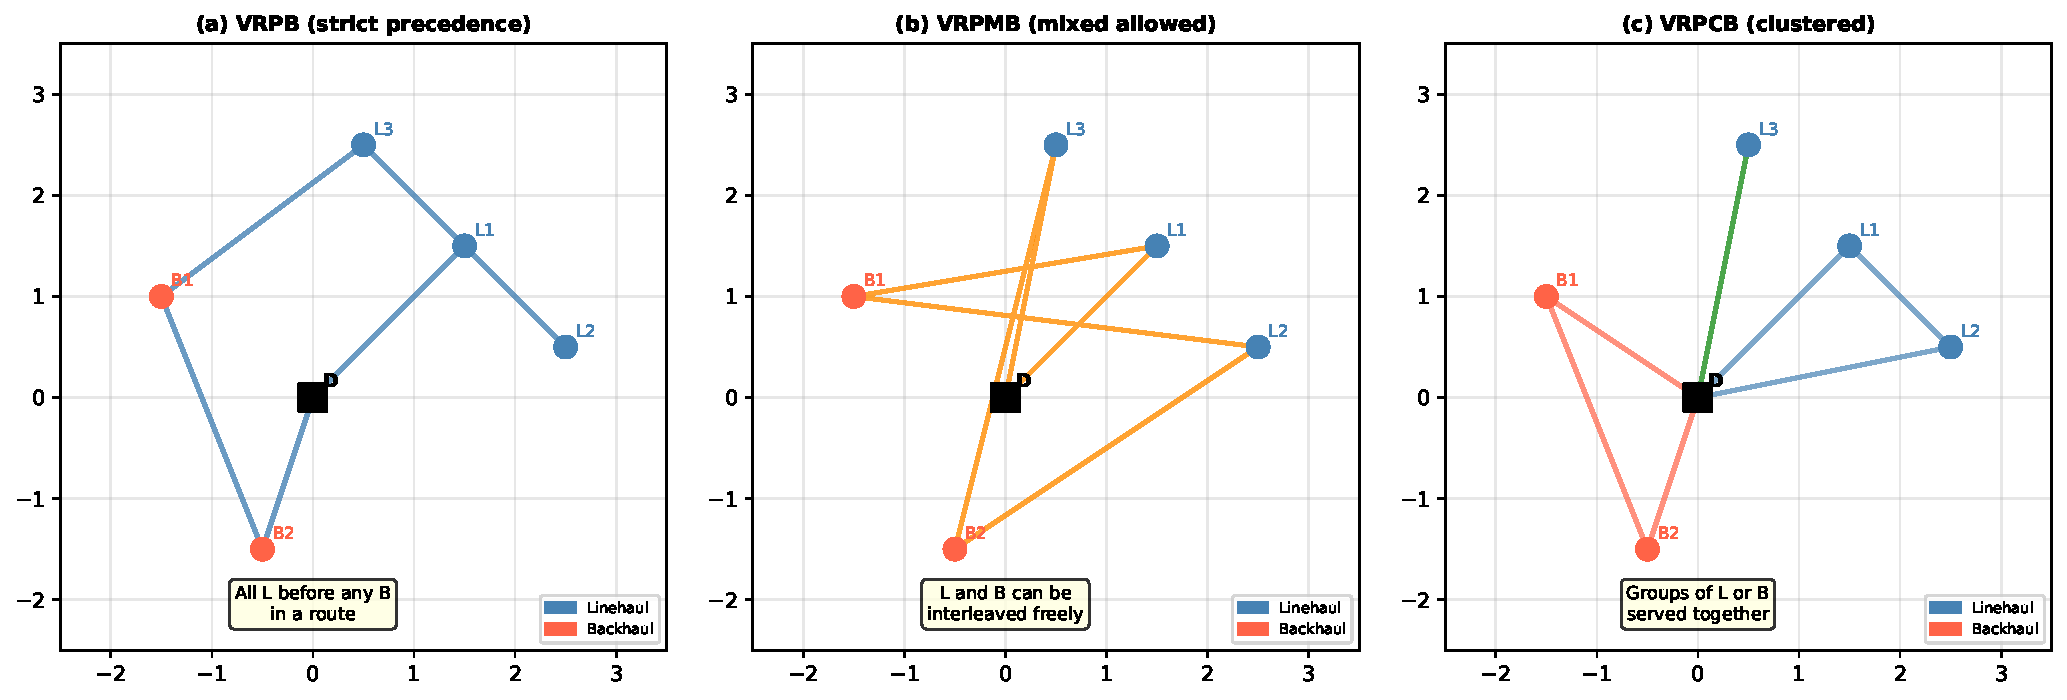
\includegraphics[width=0.88\textwidth]{vrpb_variants.pdf}
\end{center}

Panel (a): The classical VRPB with strict precedence --- all linehaul customers
(blue) appear before all backhaul customers (red) in every route.  Panel (b):
The mixed VRPB (VRPMB) allows any interleaving of linehaul and backhaul
customers.  Panel (c): The clustered VRPB (VRPCB) groups customers of the
same type in separate route segments.

\end{frame}

%%--------------------------------------------------------------------
\begin{frame}[allowframebreaks]{Chapter 9: Summary Slide}

\begin{columns}[T]
  \begin{column}{0.5\textwidth}
    \begin{block}{VRPB Key Facts}
      \begin{itemize}\small
        \item Two customer types: delivery (linehaul) and pickup (backhaul).
        \item Precedence: all deliveries before any pickup on each route.
        \item Three sub-variants: strict, mixed, clustered.
        \item Best heuristic: Tabu Search (Toth and Vigo, 1997).
      \end{itemize}
    \end{block}
    \vspace{0.3em}
    \begin{block}{HFVRP Key Facts}
      \begin{itemize}\small
        \item $T$ vehicle types with different capacities and costs.
        \item Objective: minimise fixed + variable costs.
        \item Free-fleet variant: also choose fleet composition.
        \item Benchmark: Golden et al.\ 12 instances.
      \end{itemize}
    \end{block}
  \end{column}
  \begin{column}{0.5\textwidth}
    \begin{block}{PVRP Key Facts}
      \begin{itemize}\small
        \item Planning horizon $T$ periods; frequencies $f_i$ per customer.
        \item Two sub-decisions: pattern assignment + daily routing.
        \item Benchmark: Cordeau et al.\ p-instances ($T=5$).
        \item Best method: Unified Tabu Search (Cordeau et al., 1997).
      \end{itemize}
    \end{block}
    \vspace{0.3em}
    \begin{block}{SDVRP Key Facts}
      \begin{itemize}\small
        \item Customer demand split across multiple vehicles.
        \item Lower bound on vehicles: $\lceil D/Q \rceil$.
        \item Savings: up to 50\% cost reduction for large demands.
        \item Exact B\&P handles $\leq100$ customers.
      \end{itemize}
    \end{block}
  \end{column}
\end{columns}

\end{frame}

\end{document}
